\documentclass[UTF8,a4paper,11pt,fontset=fandol]{ctexart}
\IfFontExistsTF{Droid Sans Fallback}
  {\newCJKfontfamily\cjkfallback{Droid Sans Fallback}}
  {\IfFontExistsTF{Noto Sans CJK SC}
    {\newCJKfontfamily\cjkfallback{Noto Sans CJK SC}}
    {\newcommand{\cjkfallback}{\CJKfamily{song}}}}
\usepackage[margin=22mm,headheight=15pt]{geometry}
\usepackage{graphicx,float,xcolor,amsmath,amssymb,booktabs,longtable,array,tabularx}
\usepackage[most]{tcolorbox}
\usepackage{listings,needspace,fancyhdr,enumitem}
\setlist{leftmargin=2em,itemsep=0.35em,topsep=0.4em,parsep=0pt}
\usepackage[unicode,colorlinks=true,linkcolor=blue!45!black,urlcolor=blue!45!black,breaklinks=true]{hyperref}
\usepackage{xurl}
\setlength{\parindent}{0pt}
\setlength{\parskip}{0.65em}
\setlength{\emergencystretch}{3em}
\linespread{1.14}
\raggedbottom
\pagestyle{fancy}\fancyhf{}\fancyhead[L]{月球大叔 · 访谈学习笔记}\fancyfoot[C]{\thepage}
\newtcolorbox{importantbox}[1]{enhanced,breakable,colback=blue!3,colframe=blue!45!black,title={#1},fonttitle=\bfseries}
\newtcolorbox{knowledgebox}[1]{enhanced,breakable,colback=teal!3,colframe=teal!50!black,title={#1},fonttitle=\bfseries}
\newtcolorbox{warningbox}[1]{enhanced,breakable,colback=orange!4,colframe=orange!60!black,title={#1},fonttitle=\bfseries}
\lstset{basicstyle=\ttfamily\small,breaklines=true,columns=fullflexible,keepspaces=true,showstringspaces=false,frame=single,captionpos=b}
\newcolumntype{Y}{>{\raggedright\arraybackslash}X}
\newcommand{\notetitle}{孟子立：从网络系统研究到家庭算力中心}
\newcommand{\videocoverpath}{cover.jpg}
\newcommand{\videourl}{https://www.youtube.com/watch?v=c-MnSFGTSN8}
\newcommand{\videochannel}{月球大叔}
\newcommand{\videopublishdate}{2026-07-28}
\newcommand{\noteauthors}{月球大叔、孟子立}
\newcommand{\sourceurl}{https://www.youtube.com/watch?v=c-MnSFGTSN8}
\begin{document}

\begin{titlepage}\centering\vspace*{4mm}
{\Large 月球大叔 · 访谈学习笔记\par}\vspace{8mm}
{\LARGE\bfseries \notetitle\par}\vspace{7mm}
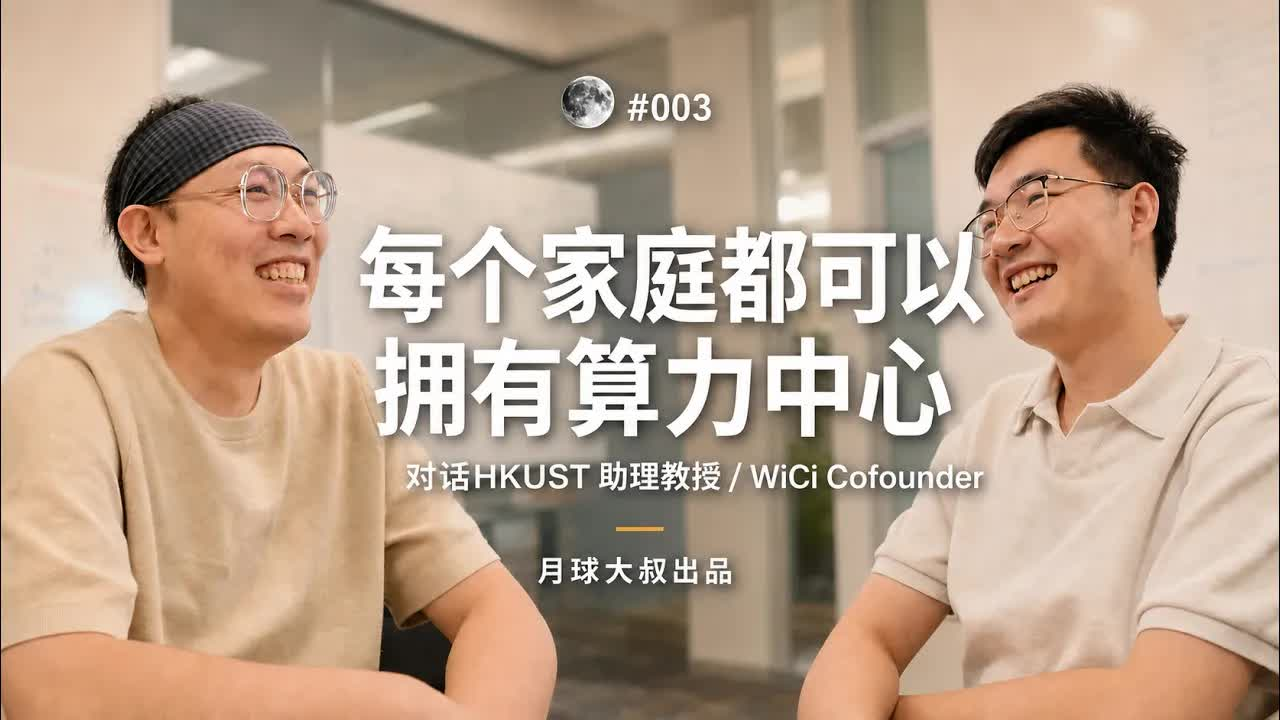
\includegraphics[width=.86\linewidth,height=.27\textheight,keepaspectratio]{cover.jpg}
\par\vspace{6mm}{\small 原节目：孟子立: 15岁，清华，HKUST，教授，家庭计算中心，云游戏，WiCi，网络系统，创业\par}
\vspace{4mm}主持人：月球大叔\par
{\small 嘉宾：孟子立\par}
\vfill YouTube 上传：2026-07-28\par
整理：2026-10-25\quad 正文：Gemini Argon\quad 配图与编校：Codex\par
\vspace{4mm}\url{https://www.youtube.com/watch?v=c-MnSFGTSN8}
\end{titlepage}
\begingroup\small\setlength{\parskip}{0pt}\tableofcontents\endgroup\clearpage
\section*{导读}\addcontentsline{toc}{section}{导读}
本笔记整理自月球大叔对香港科技大学助理教授、WiCi创始人孟子立的深度访谈。全篇沿着“问题定义—博士试错—高教培养—原型与评测—无线算力架构—商业化落地”的脉络展开：从15岁考入清华电子系、赴麻省理工学院参与强化学习与网络系统结合的早期探索，到留校直博期间通过腾讯云游戏与阿里达摩院路由器项目验证工程边界与商业时机；再到执教港科大后围绕AI时代学生选拔、论文价值与教育职能的思考。在产业转化部分，笔记拆解了AI眼镜原型暴露的硬件续航约束、实时视频通话评测平台CallArena的跨帧上下文考察，以及正在研发的家庭无线GPU方案WiCi如何借助驱动拦截、缓存、预测与调度缓解Wi-Fi弱链路代价，并聚焦“大C小B”场景与供应链协作探索商业落地。
\needspace{8\baselineskip}\section{研究从什么问题开始}
从15岁考入清华电子系到确定博士论文方向，一位年轻研究者如何找到真正值得投入的课题？孟子立在课程挫折、跨学科辅修以及麻省理工学院暑期科研的经历中，逐步从早期接触的热门算法转向计算机网络系统，并围绕日常视频通话卡顿的场景定义出跨层级的系统研究问题。
\needspace{6\baselineskip}\subsection{早期探索与应对挫折}
在访谈开篇（00:58），孟子立澄清了自己15岁进入清华大学的缘由：这并非来自清华少年班，而是因为中小学阶段就读于免去小升初与中考的学制压缩班，加上入学年龄偏早，最终以683分、高出当年录取线682分一分的成绩压线考入。高三临近高考时他的模拟考成绩曾跌出全班前十，这段波动让他形成了“降低预期、增强韧性”的心态。进入清华后，面对年龄小带来的开户、社会实践受限等生活摩擦，他在半年内逐步磨合适应；在学业上，他也把预期管理带入了高压环境中。

报道中常将他“大一选高年级课”与“微积分考70多分”混为一谈，他在节目中（04:20）特意拆开说明这是两件独立的事：高中拿过物理竞赛省一等奖的他，大一凭着冲劲在新生群看到消息就提前选修了大二的《大学物理》；而微积分考70多分则是清华电子系的普遍现象，当时班级平均分仅50多分，顶尖同学能考到98、99分。压线入学的经历让他一早接受“人外有人”的现实，没有产生剧烈的心理落差。大二时他因喜欢尝试新鲜事物报读工商管理双学位，后因学分未修满转为辅修。

这种爱折腾、愿挑战的习惯直接促成了他的科研起步（07:58）。大一下学期，面对融合了模拟电路、数字电路与电路原理的硬核课程《电子电路与系统基础》，看到任课老师在网络学堂发布招募本科生做科研的公告，他便主动报名，在实验室干了三个月的神经信号处理研究。这次机缘巧合的尝试让他顺势在大二上学期转入计算机网络方向，并因为觉得有意思而一路延续到博士阶段。

\needspace{6\baselineskip}\subsection{技术迁移、时机与系统挑战}
大三寻找海外暑期科研（暑研）时，孟子立凭借年级第一的成绩联系导师，并根据研究方向的匹配度选择了网络研究积淀深厚、曾做出数据中心传输控制协议（DCTCP）等工作的麻省理工学院 Mohammad Alizadeh 教授课题组（10:03）。他从导师视角分析，接收暑研学生对教授而言资金与试错成本很低，并非神秘的天才选拔。进组后，他跟随博士生师兄 Hongzi Mao 参与将强化学习（通过环境反馈奖励来学习决策的机器学习方法）用于网络与集群管理的研究，自己主要负责跑基线（用于对比验证新方法效果的基准实验）等实验性质的基础工作。

主持人月球大叔提到这批早期结合强化学习与系统的论文对领域影响深远，孟子立则将其归结为“时机（Timing）”与跨领域“代差套利”（12:11）。当时网络领域对新技术的应用比人工智能领域存在一两年的时间差，研究组将当时AI界热门的A3C、PPO等主流强化学习算法引入网络问题，核心创意在孟子立进组前便由 Hongzi Mao 提出。然而，把现成算法套用到大规模集群系统中绝非易事，必然会遇到大量工程与架构上的水土不服，即系统挑战。

孟子立在实践经验中强调，跨领域迁移之所以能做出成果，关键在于把算法扩展到真实系统时暴露出的那些不适配问题，逐一用脏活累活解决掉；而比埋头苦干更重要的教训是洞察力与出手时机。此后他尝试过结合AI可解释性（理解模型内部决策逻辑的机制）做网络研究并发表在顶级会议SIGCOMM上。在当时的个人探索中，他感觉到自己接触的不少AI研究围绕固定基准测试（Benchmark，标准化的评测数据集与任务）刷准确率，体验上更像解应用题；而且只要模型性能足够强、能解决实际问题，工业界与学界往往不再执着于可解释性。

\needspace{6\baselineskip}\subsection{从视频卡顿定义研究问题}
对比当时的个人科研体验后，孟子立根据自己的兴趣偏好选择了计算机网络与系统方向（14:30）。就他个人的研究体会而言，许多系统课题没有现成的固定题库或统考榜单，往往要求研究者从真实场景中定义问题（Define Question），也就是“讲故事（Storytelling）”——向审稿人清晰论证新场景的设置合理性与机制设计的巧妙之处。他坦言本科初读网络领域长达12页双栏的论文时非常痛苦，难的不是看懂字面技术，而是跨越认知差距，去理解资深学者组成的程序委员会（PC）究竟欣赏什么样的科研品味（Taste）。

围绕“系统研究核心竞争力”的话题，两位讲者在访谈中（16:16）保留了不同视角的交锋。孟子立认为，过去系统研究者引以为傲的底层编程（如编写操作系统内核或硬件驱动代码）学习曲线很陡，但在AI编程工具普及后，正如高级语言取代汇编与机器码一样，底层实现早晚会被更高层的开发方式替代，未来网络系统博士训练中最重要的或许就是讲故事的能力与系统直觉（Sense）。月球大叔则结合硅谷工业界观察指出，现阶段要想真正指挥好AI写出高质量的底层系统代码，依然需要长期的底层技能修炼，这也是目前机器学习系统工程师获得高薪的技术门槛。

落脚到自己的博士学位论文（19:00），孟子立用一个很直观的日常痛点概括了全部工作：减少微信、Zoom等实时视频通话中的网络卡顿。在这个明确的系统问题驱动下，深度学习算法只是服务于目标的辅助手段。他采取自顶向下的路径，按照计算机网络常见的TCP/IP四层结构逐层排查并消除引发延迟的因素：
\begin{enumerate}
\item 应用层：负责具体的音视频软件交互与缓冲处理；
\item 传输层：负责端到端的数据传输与拥塞控制；
\item 网络层：负责跨节点的路径选择与路由转发；
\item 链路层：负责相邻节点间的数据链路传输。
\end{enumerate}

\begin{importantbox}{科研讲故事（Storytelling）的工程实质}
在计算机系统与网络领域，“讲故事”并非虚构情节，而是问题定义与证据链构建的过程。当面对没有现成评测榜单的开放课题时，研究者需要先界定一个真实存在的系统瓶颈，说明现有方案为何在该场景下失效，再展示自己的机制设计如何消除了瓶颈，并用实验数据说服审稿人。
\end{importantbox}
\begin{knowledgebox}{计算机网络四层结构与视频延迟排查}
按照常见的TCP/IP四层视角观察，实时视频通话的数据包需依次穿过四个层级：
\begin{enumerate}
\item 应用层（视频编码与播放器缓冲策略）；
\item 传输层（拥塞控制与丢包重传机制）；
\item 网络层（跨节点路由转发与排队）；
\item 链路层（Wi-Fi等底层数据链路的接入与传输）。
\end{enumerate}
自顶向下逐层优化，意味着从上层软件交互一直排查到底层无线链路，逐一削减端到端延迟。
\end{knowledgebox}
\begin{table}[H]\centering\small
\caption{两类科研范式的个人体验对比与演进}
\begin{tabular}{>{\raggedright\arraybackslash}p{\dimexpr(\linewidth-6\tabcolsep)/3\relax}>{\raggedright\arraybackslash}p{\dimexpr(\linewidth-6\tabcolsep)/3\relax}>{\raggedright\arraybackslash}p{\dimexpr(\linewidth-6\tabcolsep)/3\relax}}
\toprule
研究维度 & 机制与任务特征 & 孟子立的早期实践案例\\\midrule
早期接触的算法打榜 & 围绕固定数据集与基准测试提升准确率等指标，个人体验类似解应用题 & 观察早期视觉、自然语言处理与强化学习刷榜后，评估觉得不符合个人长期兴趣\\[4pt]
跨领域代差迁移 & 将AI领域的新算法引入传统系统问题，重点解决规模化扩展时的系统适配挑战 & 在MIT参与Hongzi Mao构思的强化学习集群管理项目，负责跑基线与实验工作\\[4pt]
网络系统问题定义 & 从真实痛点出发定义问题，跨网络多层结构排查并消除性能瓶颈 & 博士论文聚焦减少视频通话卡顿，从应用层、传输层、网络层到链路层逐层降延迟\\[4pt]
\bottomrule\end{tabular}\end{table}
在没有固定榜单的开放场景里，研究者如何从日常痛点出发定义课题？下图梳理了孟子立博士期间将视频通话卡顿体感转化为跨层级优化方案的脉络。
\begin{figure}[H]\centering
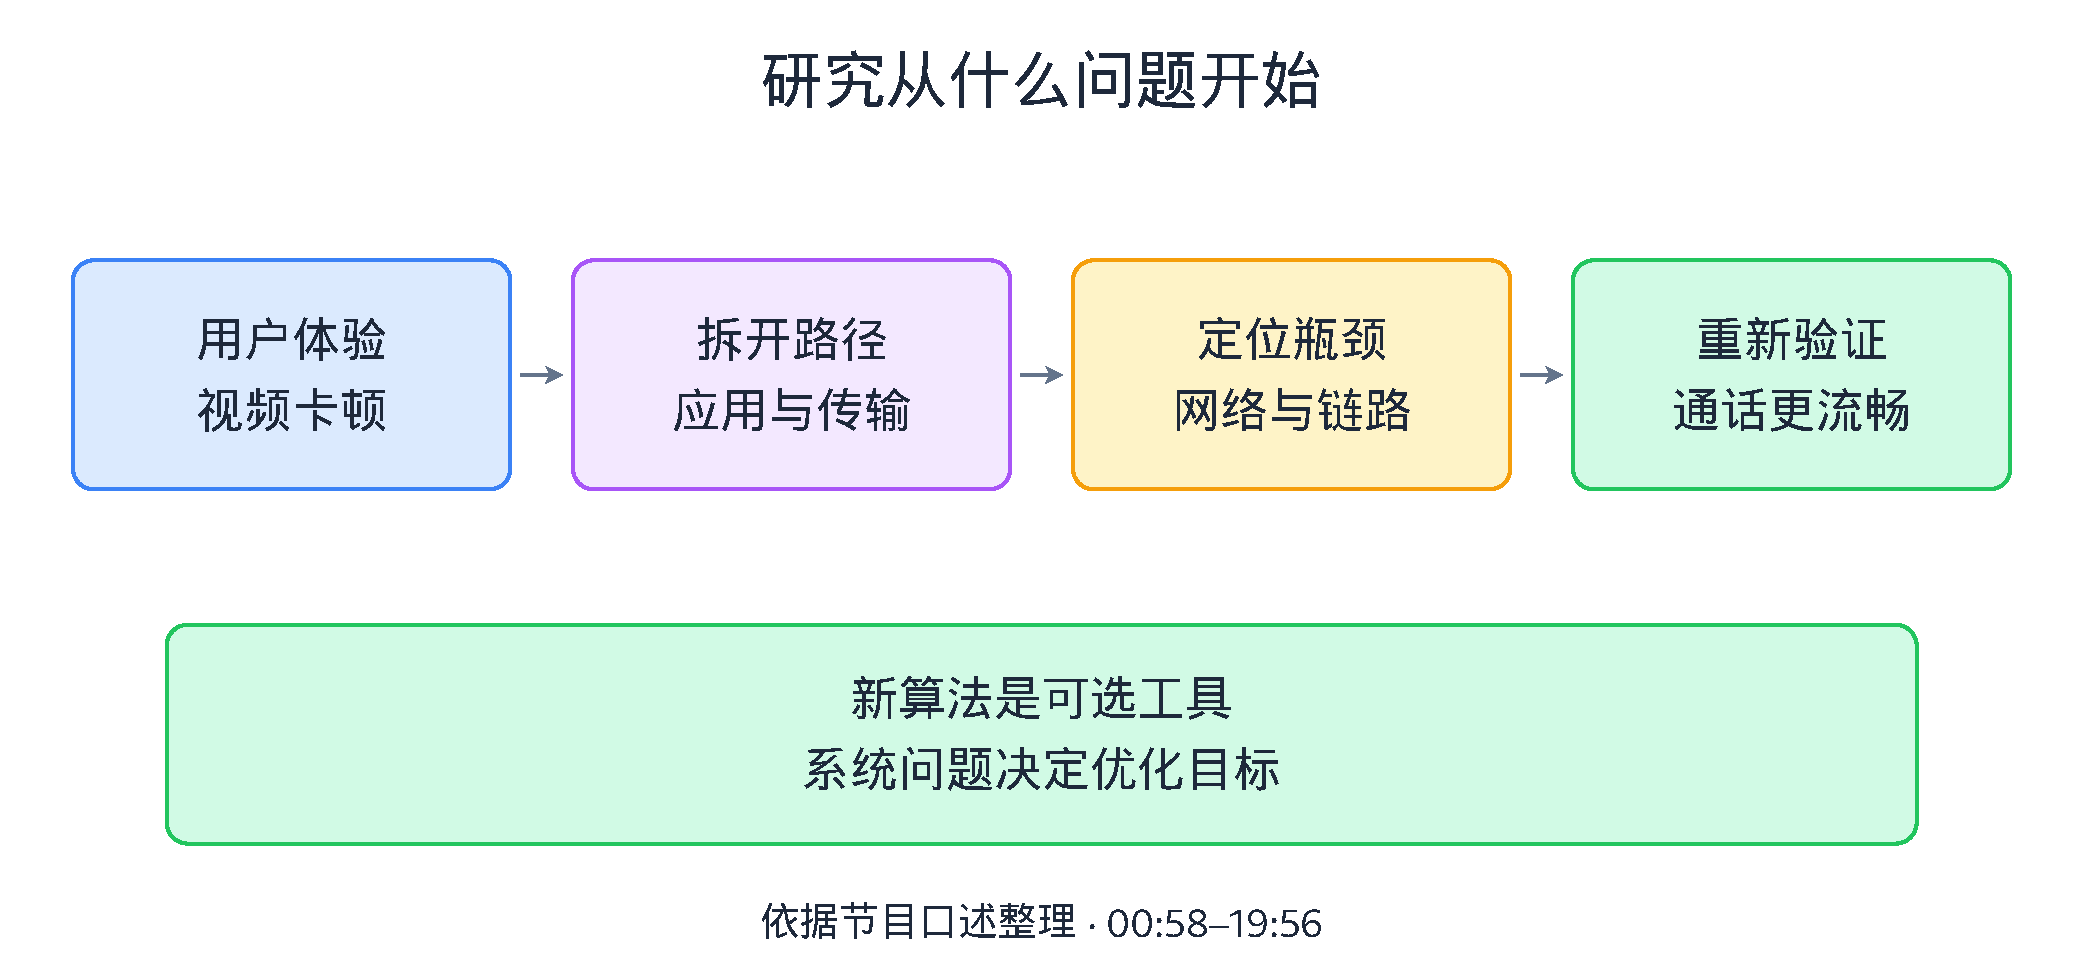
\includegraphics[width=\linewidth,height=.68\textheight,keepaspectratio]{assets/mechanism-01.pdf}
\caption{从用户体验定义系统研究问题（依据节目口述整理 · 00:58–19:56）}
\end{figure}
\begin{knowledgebox}{读图：研究从什么问题开始}
如图所示，研究起点是最左侧的“用户体验：视频卡顿”这一真实痛点；接着向右进入“拆开路径：应用与传输”，将笼统的卡顿体感拆解到应用层与传输层的具体协议与交互机制中；再向右推进至“定位瓶颈：网络与链路”，继续向下排查网络层路由与链路层传输中的延迟来源；最终到达最右侧的“重新验证：通话更流畅”，在通话场景中检验全链路优化的效果。底部横框概括了这一研究思路：“新算法是可选工具，系统问题决定优化目标”。
\end{knowledgebox}
从日常痛点出发逐层拆解问题，让机器学习算法退居为辅助工具，构成了他整个博士阶段的研究主线。
\needspace{6\baselineskip}\subsection{本章小结}
\begin{enumerate}
\item 心态与起步：降低预期、保持韧性帮助孟子立平稳度过清华电子系的学业高压，而大一主动报名实验室则开启了他的网络科研之路。
\item 时机与迁移：MIT暑研经历表明，跨领域引入新算法存在明显的时机窗口，但落地过程需要解决真实的系统适配问题。
\item 问题定义：博士论文从视频通话卡顿的真实痛点出发定义问题，自顶向下沿着应用、传输、网络与链路各层排查延迟因素，将算法作为服务于系统目标的可选手段。
\end{enumerate}
\needspace{8\baselineskip}\section{把博士阶段变成学习与试错的空间}
确定了以降低视频通话延迟为主线的研究方向后，孟子立在本科毕业时面临赴美读博还是留校深造的选择。为什么他认为博士阶段最大的误区是“只做科研”？在19:56至32:40的访谈中，他用边际分析拆解了当时的升学决策，并回顾了如何利用博士学位兜底的容错空间，在腾讯与阿里达摩院的实习中检验工程可用性与商业时机。
\needspace{6\baselineskip}\subsection{边际成本与遗漏的人脉收益}
2018年申请季正值中美贸易摩擦初显，下一届部分清华学生的签证甚至遭到撤销（19:56）。面对是否赴美读博的抉择，孟子立引入经济学中“理性人考虑边际量”的原则，对比了边际成本（Marginal Cost，即多做一步选择所需付出的额外代价）与边际收益（Marginal Benefit，即这一步带来的额外回报）。当时赴美读博的边际成本十分明确：需要暂停手头的研究，花小半年时间备考GRE和语言考试；而边际收益则取决于海外实验室在发表顶级论文上究竟比国内高出多少增量。

为了核实这一增量收益，他通过MIT暑期研修进行了实地观察。当时国内高校在计算机网络顶会上的发表数量屈指可数，但他在对比后发现，清华导师团队与MIT课题组的科研氛围差距并不悬殊，国内团队甚至有大伙像做大作业一样全情投入同一个项目的冲劲；加之他手头已有集群调度与可解释性等正在推进的课题（ongoing projects），中断半年去备考显得并不划算，因此最终决定留在清华直博。

不过孟子立在复盘时指出，当年的边际计算遗漏了一个重要变量：校友与人脉网络（进入新学府后结识的新同行与校友资源）（21:46）。一直留在同一所学校，接触到的人际关系集合相对固定；而换一个环境则能打开一整套新的连接。他坦言学生时代往往只盯着能不能做出好研究，工作后才越发体会到学术作品之外，跨圈层的同行连接同样是宝贵的隐性收益。

\needspace{6\baselineskip}\subsection{腾讯上线经验与阿里场景变化}
除了人脉维度，孟子立强调博士生容易陷入的另一个误区是“只做科研”（24:18）。在他看来，博士学位天然提供了一层兜底保障，使这段时期成为走出舒适圈、低成本试错的最佳窗口；同时，按照他当时去美国暑研时的个人观察，在美留学生除暑期通过CPT（美国允许留学生在读期间从事与专业相关实习的许可）实习外，平时往往较难因签证身份限制长期外出实习，留在国内读博则避开了这层顾虑。在四年博士生涯里，他在清华校内的时间累计只有半年到一年，其余时间先后在腾讯实习一年、在阿里达摩院实习半年、去初创公司待了几个月，并前往CMU访问一年。

不同机构的历练带来了互补的实践经验。在腾讯云游戏业务线（直接面向真实用户的生产环境团队），他体会最深的是论文原型与上线系统的距离（26:36）。发表学术论文通常先在选定的实验设置与测试样例中跑通并验证方法，而生产系统必须防范A/B测试未能覆盖的盲区，确保各类极端边界情况（corner case）不会导致服务崩溃，这要求工程设计具备极高的周密性与匠心。

在阿里达摩院的实习则让他直观撞上了商业场景与时机的约束（27:45）。当时他们做了一款旨在压低Wi-Fi尾延迟（Tail Latency，指延迟分布中较慢的那部分高分位延迟；孟子立在节目中以99\%时间正常、1\%时刻出现延迟波动来举例说明）的路由器雏形，并依托本科师兄的引荐进入阿里寻找落地场景。团队分析发现，用户不会因为刷手机淘宝直播卡顿就专门换路由器，钉钉体量太大又难以靠小测试撬动，于是将目标放在2021年家长付费意愿较强的“在线教育网课防卡顿”场景。然而入职仅三个月，“双减”政策出台，原本看好的在线教育路由器场景受挫，硬件未能上线，最终转化为一篇学术论文发表。这段经历让他切身体会到：技术能跑通只是起点，产品能否成立还取决于付费动机与外部时机。

\needspace{6\baselineskip}\subsection{支持、健康与长期投入}
如此高密度地跨界折腾，离不开导师团队的包容。孟子立与主持人交流时谈到，许多课题组并不赞成学生频繁外出实习，而他在清华跟随的毕军老师则给予了充分的支持（26:18）。在良好的团队氛围下，他得以把产业界接触到的真实问题与学术研究结合起来。

回忆起已故的毕军老师，孟子立表示自己受其科研精神影响极深（30:31）。毕军老师生前常年睡在办公室，在论文截稿日早上8点交稿前，甚至会在凌晨2点和5点分两轮给熬夜的学生发咖啡，46岁时不幸离世。那些网络研究院报道中“与时间赛跑”的细节，全是他亲历的日常。

在敬仰导师拼搏精神的同时，孟子立也谈到自己对健康的感悟：一定要高度重视身体健康（31:32）。无论是做学术还是创业，都不能靠短期高强度爆发却难以维持的方式（bursty）来推进，而要追求长期可持续的节奏（sustainable），把事业当成十年、二十年的长期过程来经营。

\begin{knowledgebox}{用边际成本与边际收益拆解升学决策}
经济学中的“边际分析”关注在现有状态上多迈一步所带来的增量变化，而非沉没成本或总体光环。孟子立在2018年评估是否赴美读博时，列出了三项关键变量：
\begin{enumerate}
\item 显性边际成本：备考GRE与语言需耗费小半年时间，并迫使手头正在推进的科研项目中断；
\item 科研边际收益：实地对比MIT与清华课题组后，判断双方在网络方向的投入氛围与产出条件差距有限；
\item 事后复盘补全的隐性收益：跨校流动带来的全新校友网络，这一点在学生时代容易被低估。
\end{enumerate}
\end{knowledgebox}
\begin{warningbox}{误区：把“论文跑通”直接等同于“产品能卖”}
学术研究原型通常先在选定的实验条件下验证核心思想要点；但走向真实产业时，技术必须跨越两道门槛：
\begin{enumerate}
\item 工程可用性门槛：生产环境（production）面临复杂多变的实际工况，要求排查各类极端边界情况（corner case），填补A/B测试未能覆盖的盲区；
\item 商业可行性门槛：即便技术指标（如抑制Wi-Fi尾延迟波动）表现良好，若缺乏用户明确的付费痛点或遭遇政策与行业时机变化，依然难以走通商业化落地。
\end{enumerate}
\end{warningbox}
\begin{table}[H]\centering\small
\caption{博士阶段三类历练的关注点与收获对照}
\begin{tabular}{>{\raggedright\arraybackslash}p{\dimexpr(\linewidth-6\tabcolsep)/3\relax}>{\raggedright\arraybackslash}p{\dimexpr(\linewidth-6\tabcolsep)/3\relax}>{\raggedright\arraybackslash}p{\dimexpr(\linewidth-6\tabcolsep)/3\relax}}
\toprule
概念/阶段 & 核心机制 & 本期案例\\\midrule
留校读博决策 & 对比显性时间投入与环境增量收益 & 省去半年语言备考继续推进在研课题，事后复盘意识到遗漏了跨校校友网收益\\[4pt]
腾讯业务部门实习 & 消除极端边界情况以保障生产环境稳定 & 参与云游戏业务上线，体会论文实验验证与生产级系统防范崩溃的差异\\[4pt]
阿里达摩院实习 & 寻找刚性付费场景并承受外部时机检验 & 针对Wi-Fi尾延迟研发路由器，选定网课场景却因2021年双减政策冲击而转为发表论文\\[4pt]
\bottomrule\end{tabular}\end{table}
为什么孟子立认为博士阶段不能只埋头写论文？下图根据19:56至32:40的访谈内容，整理了他从升学决策到企业实习试错的完整反馈路径。
\begin{figure}[H]\centering
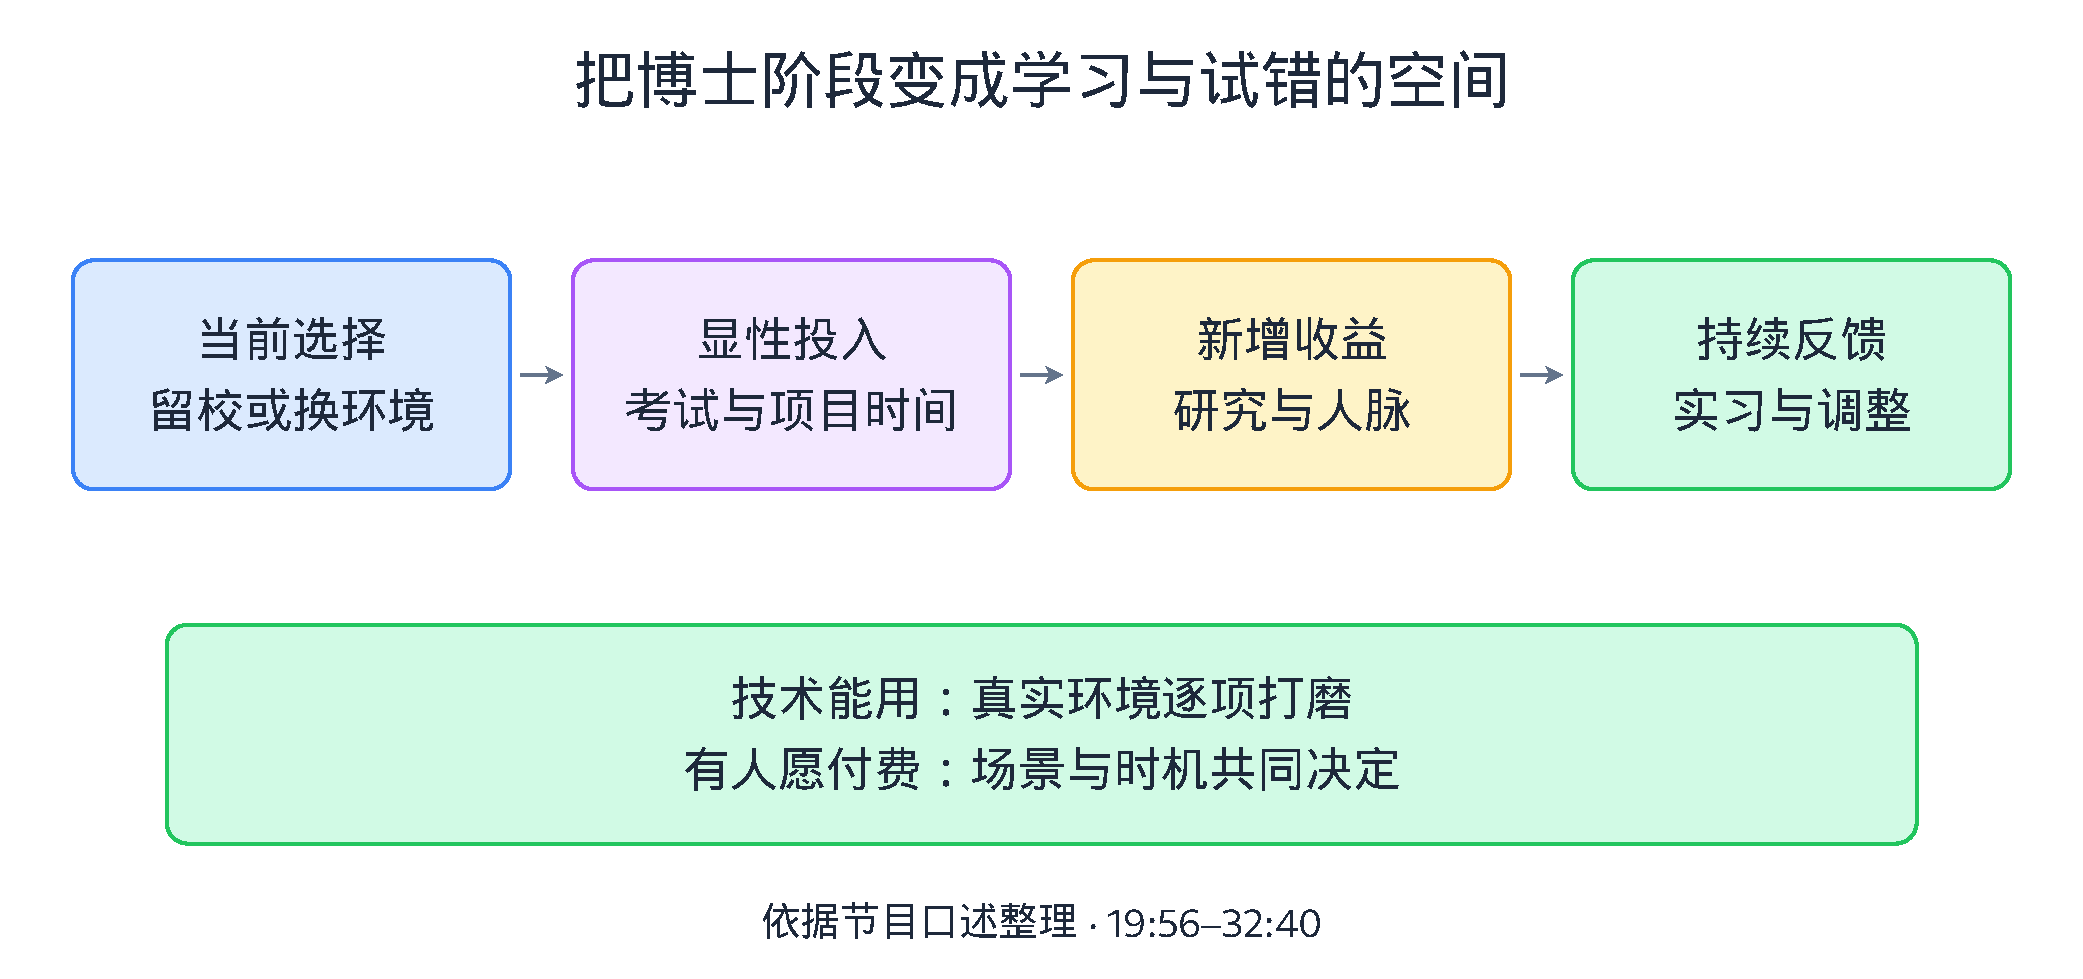
\includegraphics[width=\linewidth,height=.68\textheight,keepaspectratio]{assets/mechanism-02.pdf}
\caption{图 2-1 把博士阶段变成学习与试错的空间（依据节目口述整理 · 19:56–32:40）}
\end{figure}
\begin{knowledgebox}{读图：把博士阶段变成学习与试错的空间}
图中上方由左向右展示了四个顺次推进的环节：从“当前选择（留校或换环境）”出发，首先评估“显性投入（考试与项目时间）”，进而权衡“新增收益（研究与人脉）”，并通过“持续反馈（实习与调整）”在博士四年间不断拓展认知边界。下方汇总框则提炼出他在产业界试错后沉淀的两条核心准则——“技术能用：真实环境逐项打磨”与“有人愿付费：场景与时机共同决定”。
\end{knowledgebox}
把学位当作兜底保障，走出实验室在真实业务与商业场景中试错，帮助他在读博期间建立起对工程落地与市场时机的直观认识。
\needspace{6\baselineskip}\subsection{本章小结}
\begin{enumerate}
\item 升学评估：用边际成本与边际收益权衡留校与出国，事后复盘补充了跨校人脉网络的价值。
\item 实习试错：利用博士容错空间走访多家机构，在腾讯体会生产级系统的周密性，在阿里路由器项目中认识付费场景与政策时机的影响。
\item 长期主义：铭记毕军老师的科研热忱，同时坚持可持续的工作节奏，将身体健康作为长期投入的前提。
\end{enumerate}
\needspace{8\baselineskip}\section{AI 改变工具之后，大学培养什么}
从博士毕业走向高校教职，研究者的核心任务不再只是个人完成单个项目，而是组织团队、获取经费并培养学生。当 AI 编程工具快速降低代码实现的门槛，高校选拔和训练研究生的重心也随之转向问题判断力与自主学习能力。
\needspace{6\baselineskip}\subsection{教职选择与研究组责任}
2022 年求职季正逢疫情期间科技大厂裁员，工业界研究院岗位收缩（32:40）。当时在卡内基梅隆大学（CMU）访问的孟子立原本计划去工业界研究实验室，面对环境变化转而申请教职与博士后，最终接受了香港科技大学的录用。吸引他的一个关键因素是港科大浓厚的包容度与多元氛围：面试时他遇到无线芯片公司 Atheros 的联合创始人（后被高通收购）在系里任教，校园里既有深耕学术的学者，也有像孵化出大疆那样推动硬件创业的教授，这为日后发展保留了多种选择（35:16）。

在地域环境上，香港的科研与创业呈现出不同特点（48:57）。孟子立分享实践经验时指出，香港本地学术圈体量较小，研究经费申请（Grant Proposal）通常直接送往全球各地的同行评审，减少了人脉运作的干扰，反倒让学者能把精力集中在研究本身；但在科技创业方面，香港偏重金融属性，若涉及硬科技研发与供应链配套，毗邻的深圳以及湾区、北京等技术人才密度更高的地区具备更匹配的产业条件。

从博士生转变为助理教授，思维方式发生了两处转变（39:03）：
\begin{enumerate}
\item 追求正外部性：研究目标从发表单篇论文转向思考哪些工作更有意思、能为学术社区或他人带来积极的外部价值（Positive Externality），从而构建有影响力的研究方向；
\item 承担筹资责任：需要像创业拉项目一样申请各类科研经费（Grant），向跨领域的大同行阐述课题价值，为团队里的学生提供资金支持。
\end{enumerate}

\needspace{6\baselineskip}\subsection{按学生阶段调整指导}
随着 AI 辅助编程工具的演进，研究组选拔学生的标准也在逐年调整（37:36）。在 2023 年刚使用 Copilot 的阶段，系统方向最看重底层动手能力，孟子立曾在招生页面明确要求申请者至少写过 1000 行代码以上的项目；而当大模型能够通过自然语言指令生成大量代码后，单纯的代码行数不再是唯一门槛，他更看重系统直觉（System Sense）——即在没有固定测试榜单的开放环境里，敏锐判断哪个系统问题值得定义、哪种技术路径能够走通的能力。

在具体指导博士生时，孟子立认为不能走“大包大揽”或“完全放养”的极端（40:28）。如果导师把想法、实验和论文全部包办，学生只充当执行指令的智能体（Agent），毕业离开导师后依然缺乏独立的系统思维；反之，如果对刚入学、科研品味尚未成型的学生完全放养，学生又会在不成熟的想法里反复踩坑，陷入迷茫。

因此，合理的指导方式需要根据学生的训练基础动态演进：对刚起步、还不清楚如何开展研究的新生，导师给出明确的任务指令与及时反馈，帮其走通流程；当学生积累了一定经验、能力成长起来后，再逐步放手，通过共同探讨问题判断力，最终过渡到让学生自主探索和设计验证。

\needspace{6\baselineskip}\subsection{论文载体、认同与学习能力}
当写作、审稿甚至阅读都开始借助 AI 工具时，学术论文作为纯文字载体的意义受到了重新审视（42:06）。孟子立曾向网络顶会 SIGCOMM 社区提出过一项提案：与其只提交长篇文字论文，不如直接提交维护良好的代码库（Codebase），由官方配置 Agent 供审稿人直接向代码库提问核实细节。与此同时，在主持人月球大叔看来，把文字写清楚依然是训练大脑逻辑的必要过程；孟子立则认为，这种逻辑训练主要集中在摘要和引言的故事线梳理上。尽管如此，嘉宾强调论文仍有一项不可替代的育人价值：它为学生提供正向激励与自我认同。正如他大二第一次因海报论文（Poster）赴美参会时，不仅学术工作获得同行认可，每天 100 美元的差旅补助也带来了直接的成就感，促使他坚定了科研道路。

面对“AI 时代大学是否失去意义”的讨论，孟子立从大学的“筛选”与“培养”双重职能进行了拆解（44:46）。按他的课堂观察，排在前面的部分学生具备很强的自驱力，往往不需要老师按部就班讲授；甚至那些尝试用 AI 眼镜或工具寻找捷径的学生，至少已经在主动调用新工具想办法解决问题。在他看来，真正需要大学老师发力帮助的，是明明知道 AI 工具摆在面前却连账号都不愿注册、缺乏尝试意愿的学生。

因此，当工具自动化降低了部分执行门槛后，大学教育在培养层面的重要任务是托底并拉高学生的能力下限——促使后段学生主动接触新工具、把没试过的事情试透，培养进入陌生环境后快速吸收新知识的适应性与自我学习能力。

\begin{warningbox}{科研指导误区：把学生当执行器或过早完全放养}
在博士生培养中，常见两类极端误区：
\begin{enumerate}
\item 导师大包大揽：包办选题、设计与论文撰写，只把学生当作跑实验的执行工具，导致学生毕业后缺乏独立定义问题的系统思维；
\item 过早完全放养：对尚未建立科研品味的新生完全放手，任由其在不成熟的方向里摸索，容易在早期踩坑并陷入迷茫。
\end{enumerate}
合理的指导方式应随学生训练基础动态调整，从起步期的明确指令逐步过渡到自主探索。
\end{warningbox}
\begin{knowledgebox}{代码库审核提案与论文的双重属性}
针对 AI 参与写作与审稿的趋势，孟子立曾向 SIGCOMM 社区提议提交结构化代码库并配合智能体备询（注：这属于个人社区提案，并非会议已采纳的制度）。这一思考将学术论文拆解为两层属性：作为“信息交互载体”，纯文本部分正被代码库和自动化工具分担；但作为“逻辑训练（如撰写引言故事线）与新生成就感来源”，论文发表依然承担着学术育人功能。
\end{knowledgebox}
\begin{table}[H]\centering\small
\caption{AI 工具演进下的科研训练与高教职能转变}
\begin{tabular}{>{\raggedright\arraybackslash}p{\dimexpr(\linewidth-6\tabcolsep)/3\relax}>{\raggedright\arraybackslash}p{\dimexpr(\linewidth-6\tabcolsep)/3\relax}>{\raggedright\arraybackslash}p{\dimexpr(\linewidth-6\tabcolsep)/3\relax}}
\toprule
维度 & 传统重心或形式 & AI 时代的转变与应对\\\midrule
学生选拔标准 & 考核底层代码量（如写过 1000 行以上项目） & 弱化纯编码门槛，转向考察定义开放问题的 System Sense\\[4pt]
博士生指导策略 & 固定采用导师包办或自由放养模式 & 按阶段动态调整：从起步期明确指令过渡到独立自主验证\\[4pt]
学术成果载体 & 依赖长篇论文承载全部技术细节 & 训练引言逻辑与保留发表激励，探索代码库直接备询提案\\[4pt]
大学培养目标 & 面向全体讲授固定知识与应试技能 & 顶尖学生自主探索，重点拉高后段学生的工具使用与自学下限\\[4pt]
\bottomrule\end{tabular}\end{table}
当 AI 工具能够自动完成大量代码编写与文本处理后，导师如果只让学生机械执行指令，就失去了培养意义。下图梳理了研究生从入门到独立的培养演进机制。
\begin{figure}[H]\centering
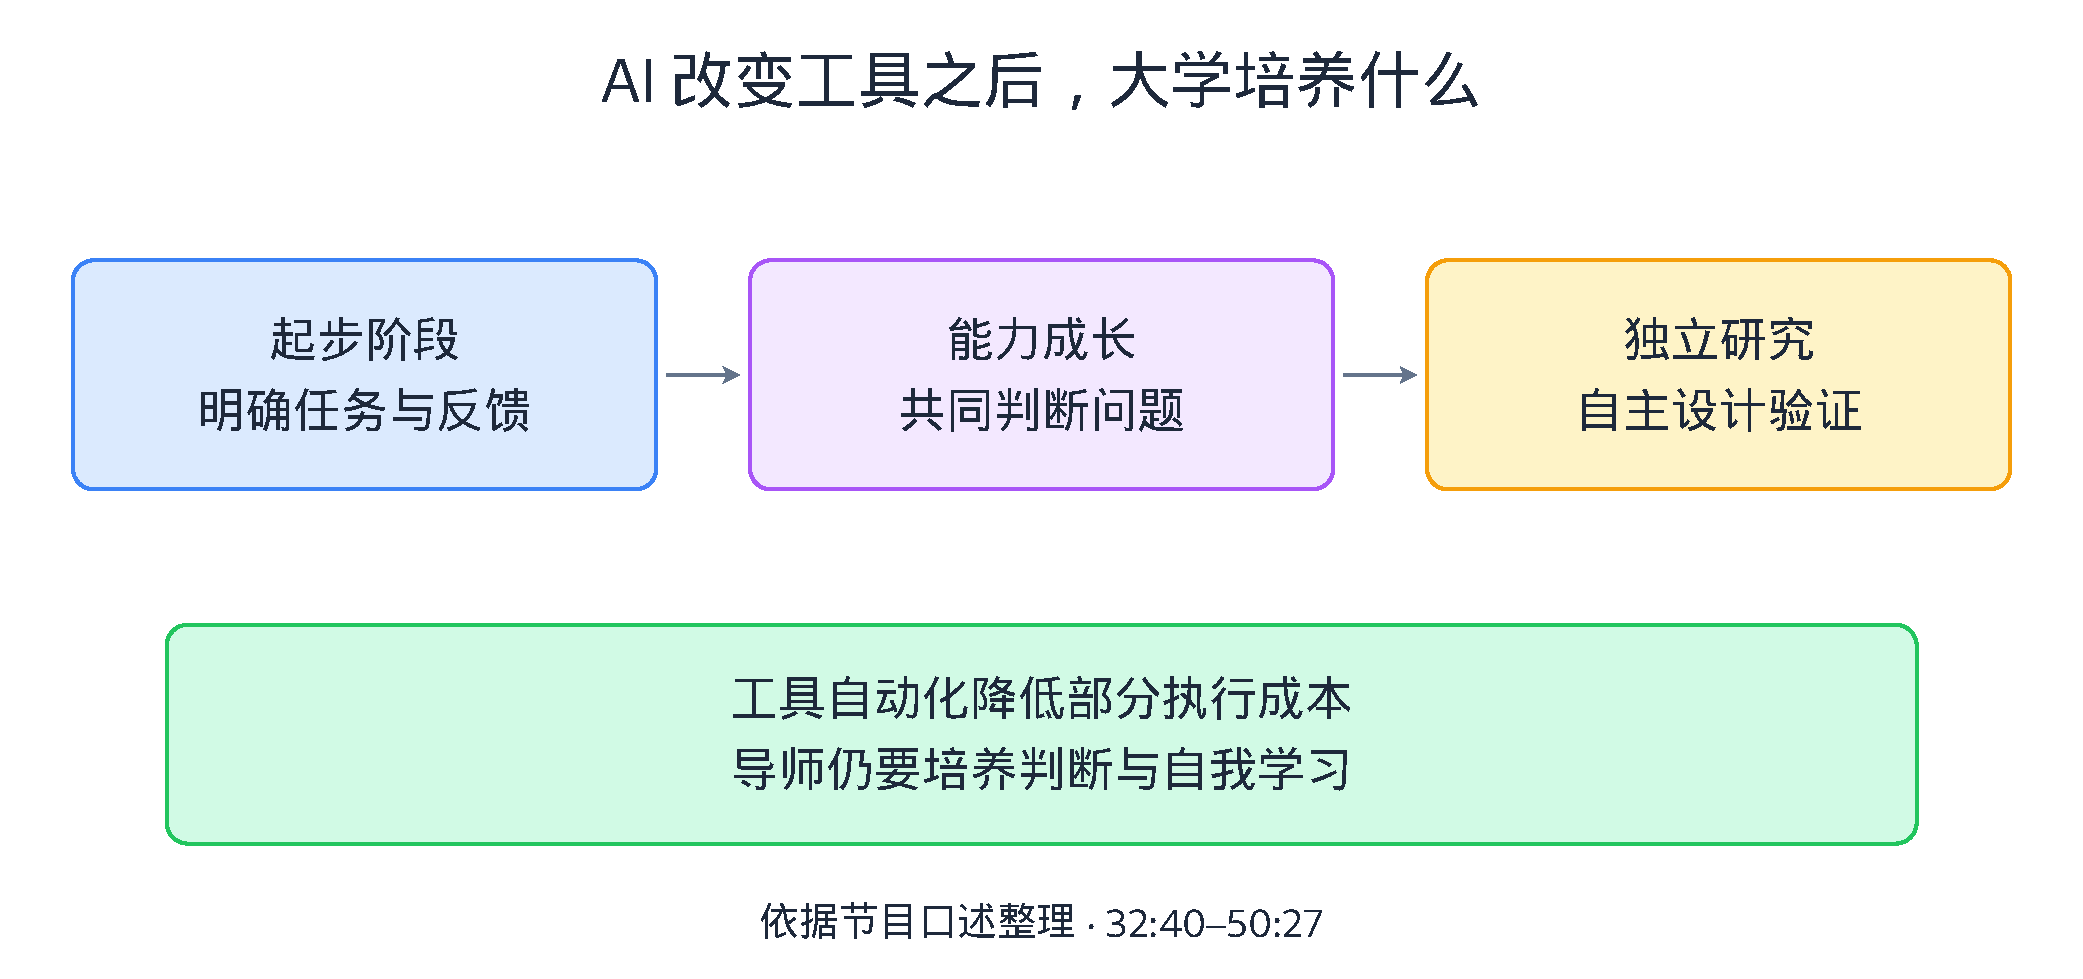
\includegraphics[width=\linewidth,height=.68\textheight,keepaspectratio]{assets/mechanism-03.pdf}
\caption{图 3：AI 改变工具之后，大学培养什么（32:40–50:27）}
\end{figure}
\begin{knowledgebox}{读图：AI 改变工具之后，大学培养什么}
图中上方三个递进节点展示了按学生阶段调整指导的过程：最左侧“起步阶段”针对科研新生，通过“明确任务与反馈”帮其建立基本规范；随着箭头指向中间的“能力成长”阶段，导师与学生转向“共同判断问题”，锤炼系统直觉；最终到达右侧“独立研究”阶段，由学生“自主设计验证”。下方横跨全局的绿色底座指出了这一演进的时代背景：尽管“工具自动化降低部分执行成本”，但“导师仍要培养判断与自我学习”。
\end{knowledgebox}
随着自动化工具分担更多底层执行工作，研究生指导与大学教育的重心进一步集中到问题判断力、工具尝试意愿以及自主学习能力的培养上。
\needspace{6\baselineskip}\subsection{本章小结}
\begin{enumerate}
\item 角色转变：从博士到助理教授，重心从单篇论文转向研究的正外部性、跨领域筹集经费与团队建设，并结合香港科研环境与深圳产业条件开展工作。
\item 选拔与指导：AI 降低了编码门槛，选才标准从“1000 行代码项目”转向 System Sense；指导学生需避开包办与放养，从明确指令逐步过渡到独立研究。
\item 教育价值：论文除承载信息外，还兼具引言逻辑训练与学生自我认同激励；大学在筛选之外，更需提升后段学生主动使用工具与适应新环境的自学下限。
\end{enumerate}
\needspace{8\baselineskip}\section{从眼镜原型到视频交互评测}
当大学教育需要回应AI工具带来的冲击时，孟子立团队直接用一场真实的考场实验把问题摆上了台面：能否做出一副看题即显答案的AR眼镜？从这个研究原型到评估大模型视频通话能力的CallArena平台（50:27–58:07），两段探索展示了系统研究者如何通过搭建原型暴露硬件约束，并设计评测指标去衡量连续交互中的用户体验。
\needspace{6\baselineskip}\subsection{眼镜让系统瓶颈变得具体}
孟子立在讲授计算机网络课程并参与监考时，看到有学生戴着墨镜进考场。由于他本身从事实时通信（RTC，对端到端延迟敏感的音视频交互技术）与可穿戴设备相关的研究，这个画面触发了他的好奇心（50:27）：如果以考场为设想场景，能否做出一副让佩戴者看向试卷就浮现答案的增强现实（AR）眼镜？团队由此启动了一个研究原型项目，目的并不是去破坏考试秩序，而是通过动手验证这种技术路径的可行性，促使教育界反思在工具变化后应当如何调整教学与考核。

真正把原型搭起来后，纸面上的设想迅速转化为一连串具体的系统挑战（52:16）。日常用手机拍照搜题时，用户可以主动对焦并把题目拍得端正清晰；但眼镜摄像头的广角视野覆盖了上下左右很大一片区域，试卷在画面里只占很小一块，不仅拍摄角度倾斜，局部清晰度也受限。更棘手的是，系统需要把识别出的题目传回后端求解，并在很短时间内让返回的答案与试卷上的对应题目匹配上。这种对超低延迟传输与结果匹配的要求，让它成了一个典型的实时通信系统研究课题。

\needspace{6\baselineskip}\subsection{识别自己的优势与产品瓶颈}
这个研究原型验证了技术可行性，也引来了媒体报道与外部投资者的关注，团队一度考虑过能否将其推向商业化（53:14）。但在深入评估整条技术链路时，孟子立发现制约产品落地的真正卡点并不在软件算法或网络传输，而在于高度集成的硬件与电池续航。当时他们从开发性与功能角度筛选了市面上三款能够支持该方案的现成智能眼镜，结果发现这类轻量级眼镜受限于体积，电池容量往往很小（孟子立以约 200 毫安时为例），一旦运行实时视频采集与通信，续航表现就会急剧下降。

面对硬件续航这一物理约束，孟子立做出了及时止损的判断（54:03）。改进微型穿戴设备的功耗与电池集成度，显然不在他作为网络系统研究者的舒适区和核心优势之内，团队因此停止了该项目的商业化推进。在嘉宾的实践经验中，这种看似半途而废的尝试本身就是一次很有价值的试错：只有亲手把原型推到接近产品的边界，才能看清整个链条的瓶颈究竟在哪一环，进而分辨哪些问题能够靠自己的技术长板解决，哪些问题应当果断放弃。

从考试眼镜的实验中跳出来，孟子立也给出了他对 AI 时代个人能力培养的推论（54:42）。他用自己小时候擅长看地图记路、但在电子导航普及后这项技能迅速贬值作类比：技术演进注定会让死记硬背或机械应试等固有技能失去原有的社会价值。当外部工具随时能给出标准答案时，真正留存下来的核心竞争力是“适应性”——即被扔进一个陌生环境后，能否保持良好的思维习惯，快速摸清规则并学会新知识。

\needspace{6\baselineskip}\subsection{CallArena 为什么要问走廊有几扇门}
沿着实时视频交互的研究主线，孟子立团队接着把目光投向了多模态大模型的评测，推出了名为 CallArena 的平台（55:48）。当时市面上已经有许多针对文本对话、静态图像理解或视频生成的评测基准，但在用户与大模型进行实时语音、视频通话的场景下，依然缺乏一套能够量化好坏的标尺。为了测试现有模型的表现，他们利用香港科技大学办公楼里酷似电影《盗梦空间》的超长走廊做了一个实验：测试者打开几款支持视频通话的通用大模型应用，举着设备从走廊一头走到另一头，最后向模型提问：“刚才一共经过了多少扇门？”

测试结果显示，当时绝大部分支持视频通话的模型在这个问题上表现都不理想（56:48）。孟子立分析，这可能是因为许多系统在处理视频流时，倾向于将其作为一帧帧独立的静态图片上传给大语言模型（LLM）或视觉语言模型（VLM）处理。而在长走廊移动的过程中，门牌号要么字迹太小，要么根本没有标记；如果系统只看单帧画面，而不能把前后帧串联成连续的视频上下文，就很难分辨当前画面里的门是刚刚数过的旧门，还是新走过的一扇门。

由于团队并不从事底层基础模型的训练，他们选择从系统评测与体验质量（QoE，从用户感受出发衡量服务好坏的评价体系）的角度切入（57:10）。CallArena 允许用户在网站上直接与不同的大模型打视频电话，针对不同系统的实时交互响应开展 A/B 对比测试，以此构建定量指标（Quantitative Metric）。正如孟子立与主持人在交流中所谈到的，合理的体验质量指标不仅能暴露跨帧连续理解等交互短板，往往还会反过来影响该领域后续算法的设计方向。

\begin{importantbox}{原型验证中的“瓶颈识别与能力对齐”}
在把学术原型推向产品的过程中，技术跑通只是第一步。以 AI 眼镜原型为例，系统研究者可以通过算法与传输优化解决小视角画面识别、低延迟回传与答案匹配，但当项目遇到微型眼镜电池容量（如约 200 毫安时量级）带来的续航瓶颈时，核心难题就转移到了硬件集成与功耗控制。孟子立强调，尽早识别出系统的真实瓶颈（Bottleneck），并评估它是否匹配团队的核心优势，是决定继续投入还是及时止损的重要依据。
\end{importantbox}
\begin{knowledgebox}{静态多模态评测与实时视频通话评测的差异}
传统的视觉语言模型（VLM）评测多关注单张图像或离线视频片段的静态问答；而在实时视频通话场景中，画面随用户移动不断变化。像“走过走廊数门”这类任务，要求系统不仅能识别单帧画面内容，还要在时间轴上维持连续的上下文状态，区分新经过的门与已数过的门，这正是 CallArena 试图通过用户实时通话与 A/B 对比测试去量化的交互能力。
\end{knowledgebox}
\begin{table}[H]\centering\small
\caption{从可穿戴原型到视频交互评测的探索对照}
\begin{tabular}{>{\raggedright\arraybackslash}p{\dimexpr(\linewidth-6\tabcolsep)/3\relax}>{\raggedright\arraybackslash}p{\dimexpr(\linewidth-6\tabcolsep)/3\relax}>{\raggedright\arraybackslash}p{\dimexpr(\linewidth-6\tabcolsep)/3\relax}}
\toprule
探索项目 & 核心系统挑战 & 关键发现与决策结果\\\midrule
AI 眼镜研究原型 & 广角画面中试卷占比小、角度倾斜；需超低延迟回传并将答案与题目匹配 & 验证了实时通信可行性，但受制于微型眼镜电池续航与硬件集成瓶颈，停止商业化\\[4pt]
导航与应试能力反思 & 外部工具（如地图导航、AI 解题）替代了原有的记忆与应试技能 & 固有技能的社会价值会随技术演进而衰减，核心是培养在新环境中快速学习的适应性\\[4pt]
CallArena 评测平台 & 长走廊移动数门等场景下，门牌微小且画面连续变化，考验跨帧上下文关联 & 通过用户实时视频通话与 A/B 对比测试建立定量指标（QoE），引导算法改进\\[4pt]
\bottomrule\end{tabular}\end{table}
为什么大模型能看懂单张照片，却在边走边聊的视频通话里数不清走廊上有几扇门？下图梳理了孟子立团队在 CallArena 中设计的测试链路。
\begin{figure}[H]\centering
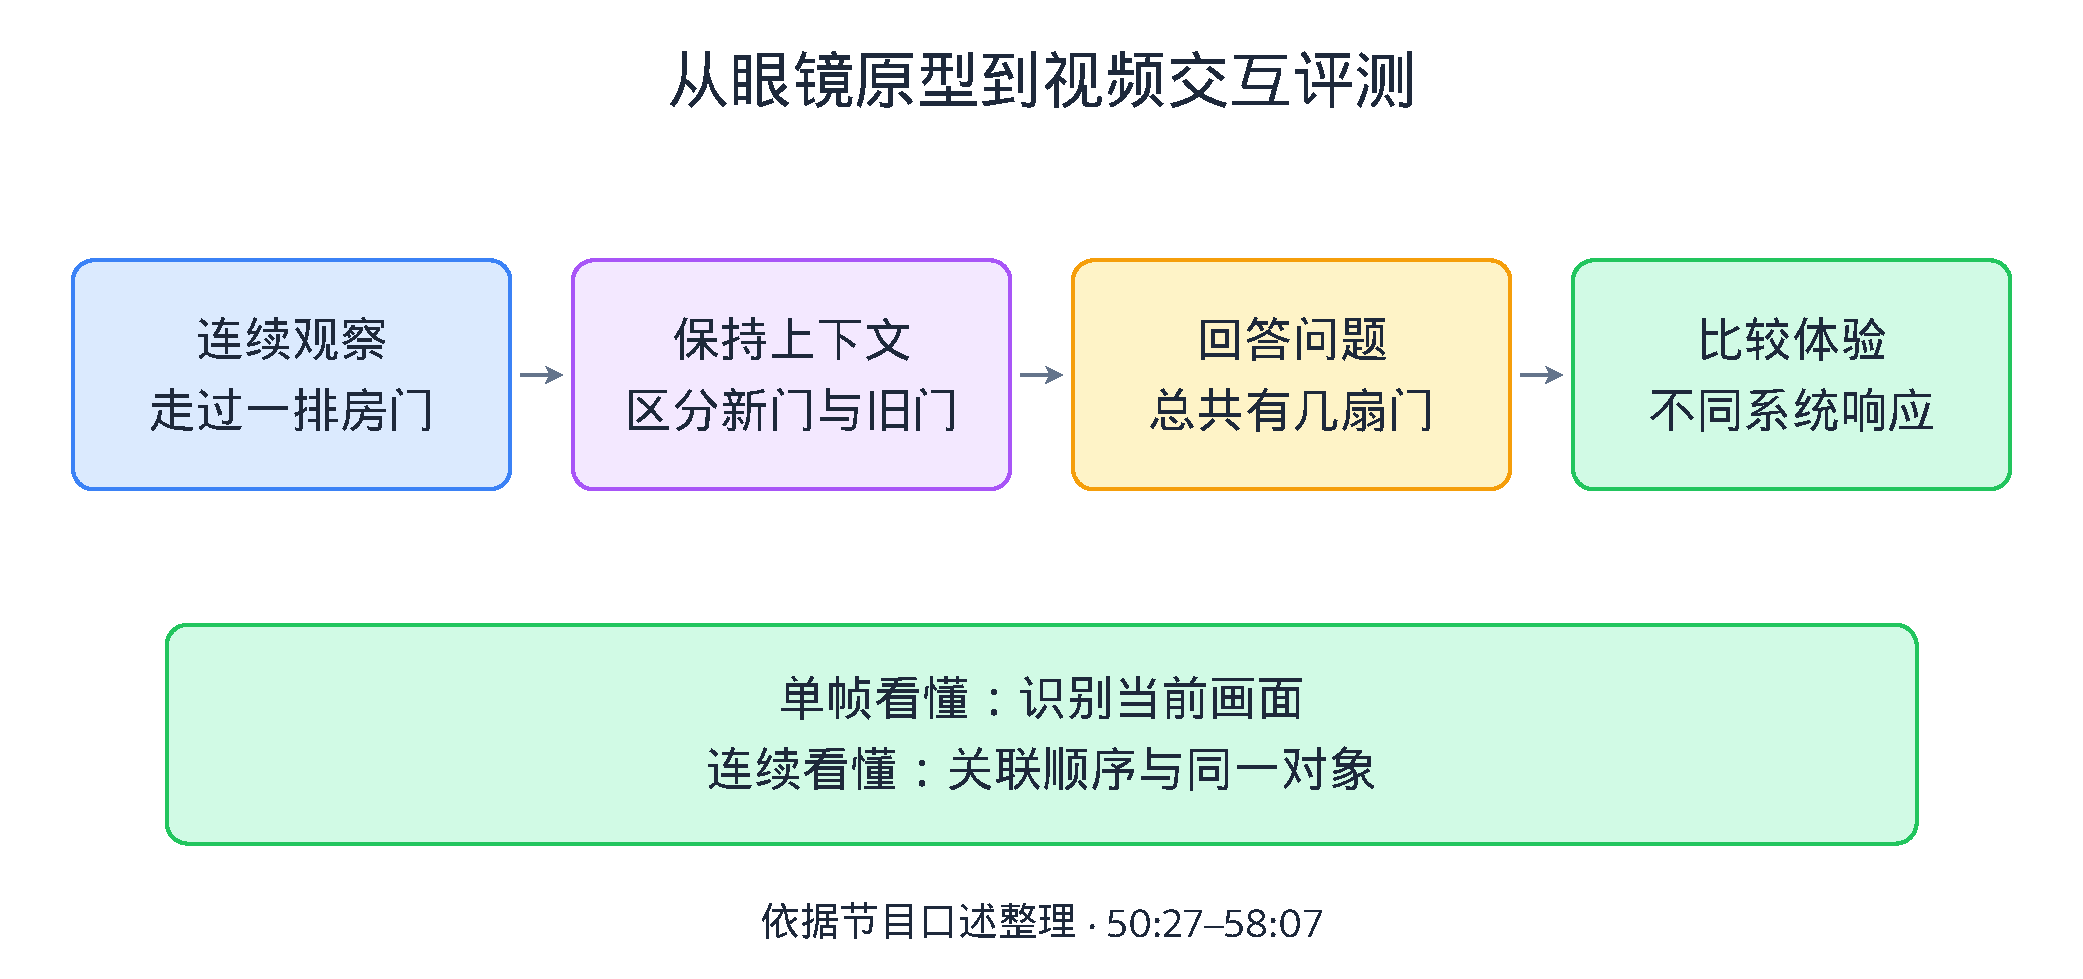
\includegraphics[width=\linewidth,height=.68\textheight,keepaspectratio]{assets/mechanism-04.pdf}
\caption{从眼镜原型到视频交互评测（50:27–58:07）}
\end{figure}
\begin{knowledgebox}{读图：从眼镜原型到视频交互评测}
如图所示，评测流程由上方四个顺次相连的节点构成：首先在“连续观察（走过一排房门）”阶段，用户手持设备沿长走廊移动并实时传输视频流；接着进入“保持上下文（区分新门与旧门）”，系统需要在移动画面中维持前后帧关联；随后到达“回答问题（总共有几扇门）”，检验模型对连续过程的累计判断；最后通过“比较体验（不同系统响应）”开展 A/B 对比测试。底部总结框指出了核心差异——“单帧看懂：识别当前画面”与“连续看懂：关联顺序与同一对象”。
\end{knowledgebox}
从动手搭建硬件原型到设计交互评测平台，这两项探索都指向同一个目标：在真实的连续交互场景中暴露系统短板，并用定量指标推动技术演进。
\needspace{6\baselineskip}\subsection{本章小结}
\begin{enumerate}
\item 原型暴露真实约束：AI 眼镜项目将考场搜题转化为低延迟传输与答案匹配问题，但也暴露出微型设备电池续航的硬件短板，促使团队认清自身优势边界并放弃商业化。
\item 工具迭代凸显适应性：如同导航取代认路，当固有应试技能的社会价值随技术演进而衰减后，人更需要保留的是进入陌生环境快速学习的适应能力。
\item 评测定义演进方向：CallArena 用“长走廊数门”检验跨帧连续理解，通过用户实时通话与 A/B 对比测试构建视频通话的体验质量（QoE）定量指标。
\end{enumerate}
\needspace{8\baselineskip}\section{无线 GPU 怎样连接家庭设备}
既然轻薄终端与穿戴设备受制于体积、重量和电池容量，无法在机身内塞入高功耗显卡，系统研究者能否换一种思路解决算力瓶颈？孟子立团队正在研发的无线算力原型方案 WiCi（58:07–65:10；70:07–75:00），尝试通过局域网一跳 Wi-Fi 与底层驱动设计，将高功耗 GPU 从移动设备中解耦出来。
\needspace{6\baselineskip}\subsection{从云游戏转向近距离共享算力}
孟子立团队构思 WiCi（Wireless Computing Infrastructure，无线计算基础设施）的起点并非大模型，而是 2024 年《黑神话：悟空》带火的高画质游戏需求（58:16）。结合此前在腾讯参与云游戏研发的实践经验，他反思了传统云端方案的局限：云游戏与云电脑通常将前端交互与后端渲染都放在远端数据中心，再把画面编码成视频流传回本地。由于公共互联网属于尽力而为（Best-Effort，不提供固定带宽与延迟保障）的网络，一旦链路跨过互联网，延迟抖动与画质损耗便很难稳定受控。

要绕开广域网的不确定性，同时解决移动设备的算力瓶颈，就必须拆解终端的物理约束。以旗舰桌面显卡 RTX 5090 为例，孟子立在访谈中提到其功耗接近 600 瓦、重量约 3 公斤，这决定了轻薄笔记本、手机或智能眼镜根本无法在机身内部塞入同等级别的硬件（59:36）。因此，团队提出将前端应用继续留在用户的本地终端上运行，仅把繁重的计算任务卸载（Offload）到家庭或办公室内仅隔“一跳”（终端与无线算力设备直接相连而不经过公网）的共享算力盒中。

在这一研发原型中，系统通过拦截驱动层函数调用（Driver-level Function Call）或应用程序接口调用（API-level Function Call），经由 Wi-Fi 发往近端算力盒执行（59:14）。按照孟子立描述的设计目标，这种改造结合了 Wi-Fi 驱动与 GPU 驱动，旨在让本地终端上的应用程序以为本机直接连着一块高性能显卡（如 RTX 5090），从而在不专门修改上层应用代码的情况下调用远端算力（01:00:21）。

\needspace{6\baselineskip}\subsection{弱链路下的驱动、缓存与调度}
把显卡从主板插槽搬到无线路由器旁，核心技术阻力来自通信链路的剧烈降级。在传统计算机体系结构中，CPU 与 GPU 通过 PCIe（Peripheral Component Interconnect Express，高速串行计算机扩展总线标准）直接相连，具备上百 Gbps 的高吞吐带宽与微秒级（\(\mu\)s）的超低延迟（01:13:08）。一旦改用家庭 Wi-Fi 替代 PCIe 总线，物理链路的可用带宽与传输延迟都会劣化数个数量级。如果直接照搬原有的图形与计算调用方式，大量时间将被消耗在无线收发等待上。

为了在弱链路（Weak Link）上维持可用性能，孟子立将这一问题重新定义为“CPU 与 GPU 通过弱链路连接的计算机体系结构问题”（01:13:34）。他回顾道，在二十多年前 PCIe 标准尚未普及的时期，消费级主板同样面临设备间通信受限的困扰。团队的解决思路是深入到底层的 Wi-Fi 驱动（Wi-Fi Driver）、GPU 驱动（GPU Driver）以及推理引擎（Inference Engine）内部，把计算机体系结构数十年的经典优化机制重新引入无线场景（01:10:25）。

在访谈中，孟子立点出了团队在底层采用的“缓存（Cache）、预测（Prediction）与调度（Scheduling）”三类优化方向（01:14:15）。结合计算机体系结构的常见机制，可以从三个层面来理解这类弱链路优化的工程逻辑（注：以下具体细节为体系结构领域的通用机制解释，并非受访者公开的内部代码实现）：
\begin{enumerate}
\item 缓存（Cache）：将频繁复用的数据或中间状态驻留在近端算力侧或本地内存中，减少在无线信道上反复搬运相同数据；
\item 预测（Prediction）：根据上下文提前预判应用接下来的调用需求，变被动等待为主动预取；
\item 调度（Scheduling）：合理安排计算与传输任务的执行顺序，尽量掩盖无线通信往返带来的等待开销。
\end{enumerate}
依靠驱动层与推理层的这些软件优化，团队希望在不自研定制芯片的前提下，尽量缓解无线连接相比板载总线的性能落差。

\needspace{6\baselineskip}\subsection{本地数据与机器人提出哪些需求}
除了高画质游戏，本地大体积数据处理与智能体（Agent）的演进也为近距离共享算力提供了潜在需求。主持人月球大叔结合自身剪辑数百 GB 视频并搭建 NAS（网络附属存储）的经历指出，将海量原始素材上传到公有云处理的传输耗时难以接受（01:01:33）。孟子立进一步补充，当前的编程辅助工具（如 Cursor、Claude Code）之所以流畅，是因为代码属于纯文本，可以直接用本地检索工具（如 grep）快速扫描；但当未来 AI 智能体深入处理家庭电脑里上百 GB 的演示文稿、文档、图片和音视频等非纯文本数据时，如果需要对海量本地文件逐一执行向量化嵌入（Embedding，将数据转换为数值向量表示以便模型检索和理解的过程），轻薄设备将面临很大的计算开销（01:02:11）。这构成了他眼中“生产力终端与算力设备解耦”的切入点。

在孟子立的设想中，这一架构同样可以延伸至家庭具身智能（Embodied AI）与家用机器人。无论扫地机器人还是未来的家务机器人，其机身只要处于移动状态，就会受到电池容量与自重的严格制约。他指出，目前机器人常见的机载计算板（如 NVIDIA Jetson Orin，或未来更强的 Jetson Thor）受限于移动端功耗，其算力增长空间难以与数百瓦功耗的桌面级或专业级显卡相比（01:04:24）。如果将家庭内部的算力盒作为共享算力来源，让屋内的移动设备通过 Wi-Fi 调用算力，终端就有望在保持轻量化的同时使用更大的模型。

目前，WiCi 团队已制作出包含迷你主机（Mini PC）、高规格显卡与无线路由模块在内的硬件原型，并正与部分机器人团队展开初步接触，希望探讨当可用算力提升 10 倍乃至 100 倍的假设下，机器人能获得何种实际增益（01:04:47）。面对创业初期资金与精力的双重约束，孟子立强调团队必须排定优先级：将核心研发聚焦在驱动与推理基础设施上，而把硬件生产交由 ODM（原始设计制造商）合作，把上层具体应用留给更懂垂直场景的开发者社区共同探索（01:10:40）。

\begin{importantbox}{机制拆解：为什么在驱动层拦截 GPU 调用}
如果为无线算力盒单独定义一套全新的应用开发接口，意味着现有的游戏、视频剪辑软件和本地工具都需要修改代码才能运行。根据孟子立在节目中的介绍，WiCi 原型的设计思路是在 Wi-Fi 驱动与 GPU 驱动层拦截函数调用或 API 调用，将其转发至局域网内的算力盒执行，目标是让上层应用以为本地直接连着一块高性能显卡。需要说明的是，这一方案目前处于研发与原型迭代阶段，“无需适配上层应用”属于受访者阐述的系统设计目标。
\end{importantbox}
\begin{warningbox}{常见误区：软件优化不能抹平无线与总线的物理代差}
阅读无线 GPU 方案时，容易误以为修改驱动后家庭 Wi-Fi 就能达到与主板 PCIe 相同的物理速率。实际上，PCIe 拥有上百 Gbps 带宽与微秒级延迟，而无线信道受限于频谱资源与环境干扰，物理性能存在数量级差距。驱动层的缓存、预测与调度机制并非改变了无线电波的传输速度，而是通过减少冗余数据传输、提前预取和重排任务来缓解弱链路的等待代价。此外，该方案目前处于研发与原型迭代阶段，上层应用的透明访问属于系统设计目标。
\end{warningbox}
\begin{table}[H]\centering\small
\caption{三种算力供给模式的系统特征对比}
\begin{tabular}{>{\raggedright\arraybackslash}p{\dimexpr(\linewidth-6\tabcolsep)/3\relax}>{\raggedright\arraybackslash}p{\dimexpr(\linewidth-6\tabcolsep)/3\relax}>{\raggedright\arraybackslash}p{\dimexpr(\linewidth-6\tabcolsep)/3\relax}}
\toprule
算力模式 & 数据传输路径 & 主要系统约束\\\midrule
本地终端内置算力 & 板载总线或芯片内部互连 & 移动设备受机身重量、散热与电池功耗墙严格限制\\[4pt]
云端远端算力（如云游戏） & 跨公共互联网传输音视频流 & 广域网尽力而为传输，延迟抖动与大文件上传开销大\\[4pt]
家庭近距离无线算力（WiCi 原型） & 局域网一跳 Wi-Fi 传输驱动级请求 & 无线带宽与延迟弱于 PCIe，依赖缓存、预测与调度缓解\\[4pt]
\bottomrule\end{tabular}\end{table}
当笔记本、手机或家用机器人受限于体积与电池，无法内置高功耗显卡，而跨互联网的云端渲染又面临延迟波动时，系统该如何重新组织本地算力调用？
\begin{figure}[H]\centering
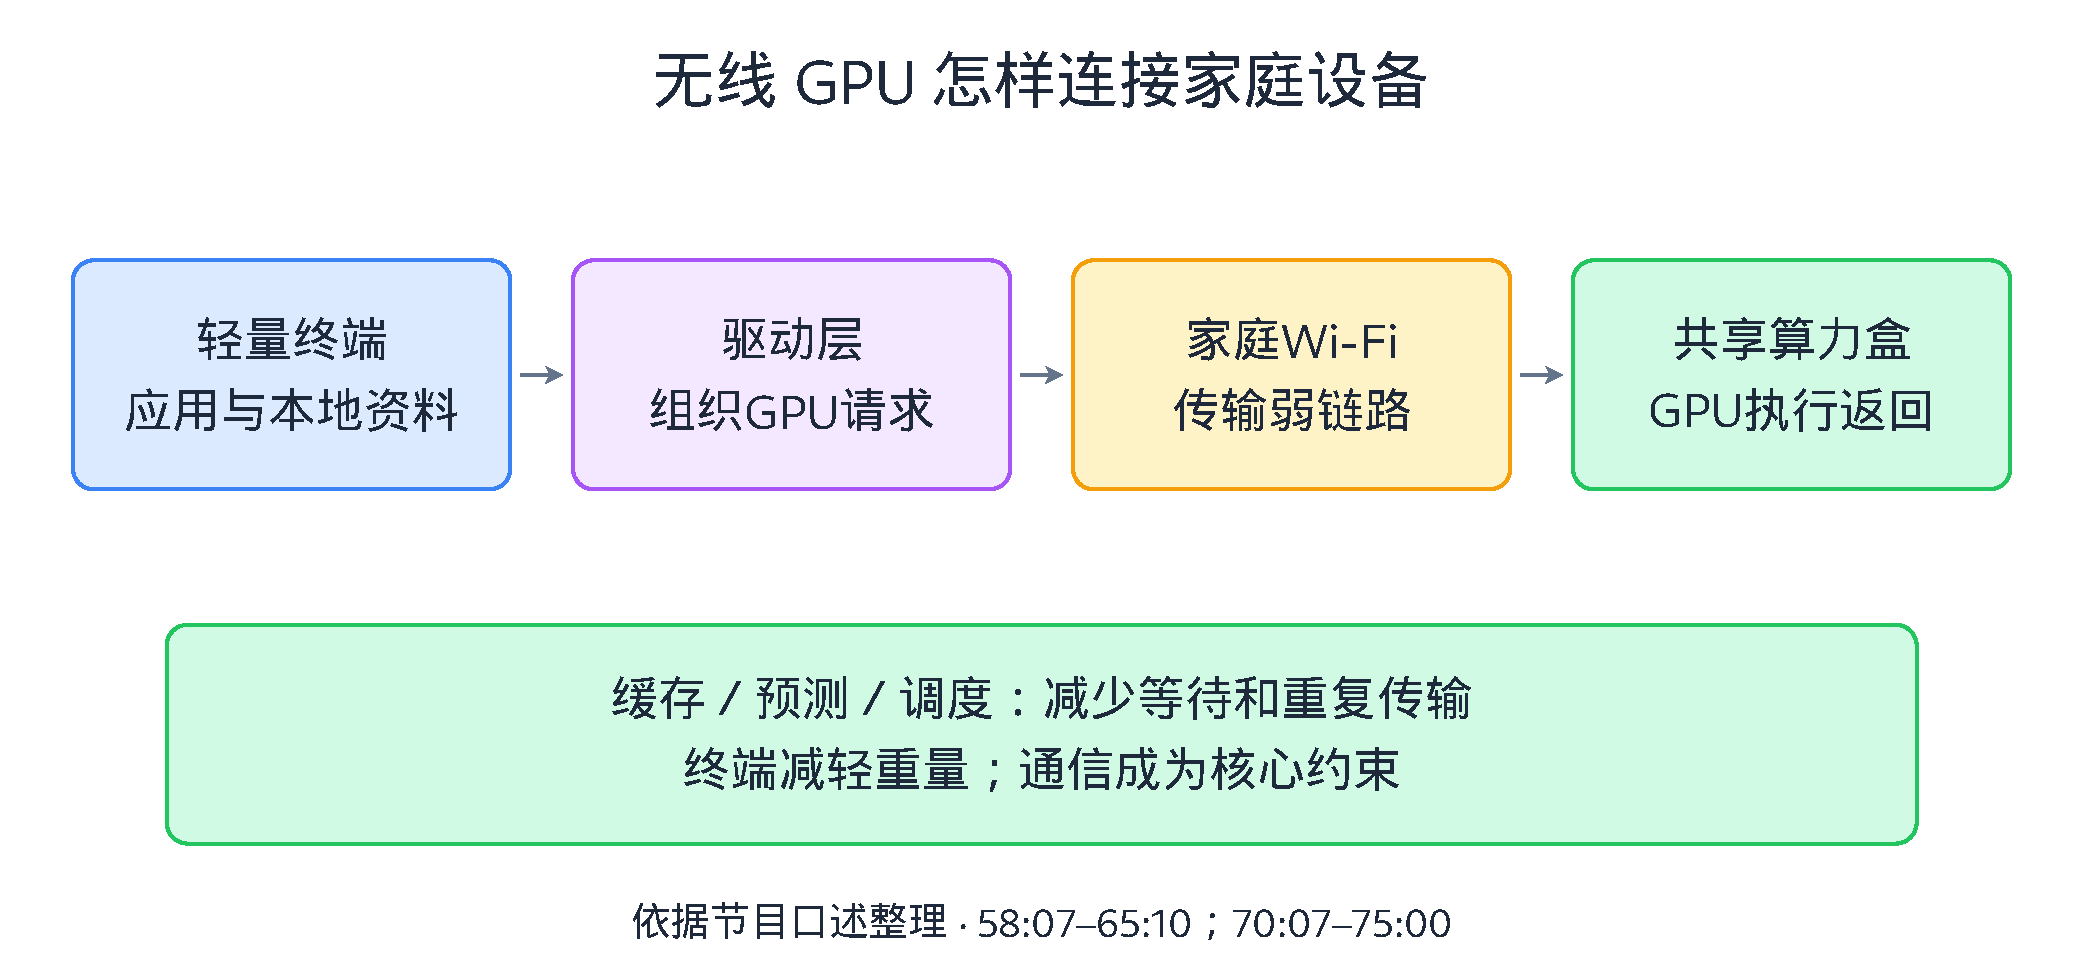
\includegraphics[width=\linewidth,height=.68\textheight,keepaspectratio]{assets/mechanism-05.pdf}
\caption{无线 GPU 连接家庭设备的机制示意（依据节目口述整理 · 58:07–65:10；70:07–75:00）}
\end{figure}
\begin{knowledgebox}{读图：无线 GPU 怎样连接家庭设备}
如图所示，调用链路从左至右分为四步：首先，“轻量终端”保留前端“应用与本地资料”，不承担重度计算；接着，请求进入“驱动层”，由系统底层“组织GPU请求”并完成拦截封装；随后，指令与数据跨过“家庭Wi-Fi”这一“传输弱链路”发往近端；最终由“共享算力盒”完成“GPU执行返回”。图下方的横幅指出了支撑整条链路运转的系统关键：由于“终端减轻重量；通信成为核心约束”，底层必须依靠“缓存／预测／调度：减少等待和重复传输”，才能弥补无线连接相比板载总线的性能落差。
\end{knowledgebox}
上述根据访谈口述整理的机制图，展示了将高功耗显卡留在固定位置、通过底层驱动与体系结构优化为局域网内多终端提供算力的原型思路。
\needspace{6\baselineskip}\subsection{本章小结}
\begin{enumerate}
\item 架构解耦：针对云游戏跨公网延迟难保障、移动端无法内置约 600W 级桌面显卡的矛盾，WiCi 原型提出保留本地前端、通过一跳 Wi-Fi 卸载计算的设计思路。
\item 弱链路优化：面对 Wi-Fi 相比 PCIe 的带宽与延迟劣势，团队将其定义为弱链路连接的计算机体系结构问题，在驱动与推理层引入缓存、预测和调度机制以缓解通信开销。
\item 场景与分工：本地海量非文本文件的处理与家庭机器人构成了潜在探索方向；团队在研发中聚焦底层驱动与推理引擎，而将硬件制造与上层应用分别交由 ODM 厂商和开发者社区协作。
\end{enumerate}
\needspace{8\baselineskip}\section{技术优势怎样变成有人购买的产品}
底层驱动与弱链路优化让无线GPU原型跑了起来，但正如孟子立在阿里达摩院路由器项目中体会到的，技术跑通不等于商业成立。在65:10至70:07及75:00至85:13的访谈中，他进一步分享了初创团队如何从宽泛的连接设想中寻找早期买单人群、划分18个月的研发优先级，并在深圳供应链试错与跨界合作中维持长期的创造状态。
\needspace{6\baselineskip}\subsection{从大量场景筛出明确付费需求}
从实验室原型走向商业公司，第一步是区分“技术上能连”与“商业上有人愿买”。WiCi这一名称将Wi-Fi中的“Fi”替换为“Ci”（Computing Infrastructure，计算基础设施），孟子立的长期愿景是让它像家用路由器一样进入家庭与办公室，成为服务各类终端的算力路由器（01:07:25）。但他也强调，能连Wi-Fi的设备虽多，却必须认清“场景多不代表应用多，应用多不代表付费意愿多”的现实（01:08:55）。如果一开始就直接面向普通大众消费者铺开，验证需求的周期会非常漫长。

因此，团队在短期商业策略上将目标锁定在“大C小B”（愿意尝鲜的专业个人用户与小型商业团队）作为早期切入口。月球大叔在访谈中从个人体验出发举了一个例子：日常剪辑视频动辄产生几百GB本地素材，传上云端处理耗时过长；若本地局域网有一台算力设备能跑开源模型辅助画质处理与切分镜头，像他这样习惯使用NAS的创作者会有意愿购买。孟子立也表示，无论是这类懂技术的极客与专业创作者，还是小型视频剪辑工作室，都是团队现阶段重点瞄准的早期目标客户（01:08:17）。

至于更广泛的线下与行业场景，比如主持人在交流中联想到的北美超市比价购物车、餐厅服务机器人等，孟子立认为开放发散能想出很多方向，但落到实际商业化上，必须配合市场推广（Go-to-Market）一步步试错。团队希望通过不断接触各类潜在场景，让更多用户意识到无线算力基础设施的实际用处；在他看来，哪怕构想的十个愿景里最终有一个真正跑通并产生社会价值，就已经是很不错的早期成果（01:11:32）。

\needspace{6\baselineskip}\subsection{把精力放在驱动与推理基础设施}
确定了早期目标方向后，初创团队紧接着要回答“未来18个月把有限的资金和时间投向哪里”。无线算力盒横跨了系统软件、无线通信与整机硬件，如果从头自研主板、外壳乃至控制芯片，战线会拉得过长。孟子立从系统研究者的角度指出，做系统的人虽然习惯于多组件协同（Multi-component Coordination），但创业必须排定优先级（Priority）（01:10:10）。

基于这一判断，团队划定了明确的研发边界与分工模式：
\begin{enumerate}
\item 核心自研层：将团队主要精力集中在底层技术上，包括Wi-Fi驱动与GPU驱动、推理内核（Inference Kernel）与推理引擎（Inference Engine），以及针对弱链路通信的性能优化；
\item 硬件制造层：不组建庞大的硬件团队，而是将“迷你主机+显卡+无线路由器”形态的整机硬件交由ODM厂商（原始设计制造商）合作生产；
\item 上层应用层：与开发者社区合作，邀请更懂垂直业务的伙伴（如机器人开发者）共同探索算力放大后的具体应用（01:10:40）。
\end{enumerate}

当被问及如果大公司或传统路由器、NAS厂商模仿该产品时如何应对，孟子立将竞争策略拆解为短期与长期两个阶段（01:12:13）。他认为，大公司推动此类跨界新产品通常需要战略层面的决策，很难仅靠自下而上快速启动；因此初创团队在短期内必须拼速度和底层性能，依托自2024年以来在弱链路体系结构优化上的积累，让竞争对手即便通过ODM做出相似的硬件盒子，也难以迅速达到同等的性能表现。而在长期维度上，他认同伟大的产品最终不能只靠单一技术赢下市场，必须依靠生态伙伴与应用价值来构建护城河（01:14:38）。

\needspace{6\baselineskip}\subsection{供应链、合作与可持续的创造}
即便把硬件制造交给合作伙伴，作为大学老师跨界创业，跑通从原型机到稳定供应的链路依然需要从头学起。回看早期做AI眼镜研究原型时，团队就曾遇到硬件与供应链难以跑通的困境（01:15:11）。到了WiCi阶段，初创公司最大的困难在于采购量小，很难单靠自下而上的常规商务流程推动合作。孟子立总结的实践经验是“把自我（Ego）放小、增强韧性（Resilience）、主动开口求助（Reach out）”：就像他刚做助理教授前两年连续写20份经费申请才中1份那样，创业找供应链、找联合创始人、找市场资源，都要主动通过投资人、朋友与亲友引荐来打通自顶向下的资源节点（01:05:23）。

在具体硬件迭代中，深圳密集的硬件生态为团队提供了很高的试错效率。由于WiCi硬件上相当于将Mini PC、GPU与Wi-Fi路由器集成到一起，开发过程中常遇到线材适配、版型与内部空间紧凑等细节问题。在深圳，一旦发现某根连接线插不上或空间放不下，联系供应商后通过跑腿闪送，往往一小时就能拿到新型号线材继续测试（01:15:11）。而在供应链踩坑回顾中，孟子立提到除起订量小之外，当时遇到的另一大困扰是高端消费级显卡（如RTX 5090）的价格波动；他事后复盘觉得，针对这类核心元器件，若能提前囤货或签署长期供应协议，在应对价格调整时会更主动（01:17:52）。

从工程管理再往深处看，不论是打通供应链、做学术研究还是推进创业，都离不开人与人的合作。孟子立反思自己15岁上大学以来吃过最多的苦其实在于磨炼性格（Personality）：从青春期相对张扬的状态，慢慢学会换位思考与对齐共同利益（Common Interest）——无论是探讨前人的学术工作还是寻找商业伙伴，都不能受情绪影响，而要站在对方角度找到能把事情做成的交集（01:20:04）。面对未来，他用“向前看，别回头”勉励自己，并强调无论做什么都是持久战，感到倦怠（Burn out）或痛苦时要懂得停下来留出缓冲空间，在保证健康的前提下享受当下的每一分每一秒；他最大的愿望，是未来人们能通过像WiCi这样有价值的代表性工作记住他的贡献（01:23:18）。

\begin{warningbox}{场景泛化陷阱：连接能力不等于购买意愿}
通用基础设施创业容易陷入的一个误区，是把“技术上能连接的设备范围”直接等同于“现成的付费市场”。只要终端支持Wi-Fi就能调用本地GPU，这界定的是技术覆盖面；但场景多不代表应用多，应用多也不代表付费意愿多。初创团队需要通过市场推广（Go-to-Market）不断试错，先从对本地算力有迫切需求的专业个人或小型工作室（大C小B）切入，在真实任务中验证用户痛点与买单意愿。
\end{warningbox}
\begin{importantbox}{深科技初创团队的“核心—外围”资源分配法}
面对软硬件交织的系统工程，初创团队受限于资金与18个月的时间窗口，需要明确划分研发与协作边界：
\begin{enumerate}
\item 聚焦底层基础设施：将团队主要精力投向Wi-Fi驱动、GPU驱动、推理内核与推理引擎等底层软件优化；
\item 借力ODM与敏捷供应链：整机硬件交由ODM厂商合作，依托深圳硬件生态快速完成线材与版型试错；
\item 联合开发者社区：将机器人等上层垂直应用交由更懂业务场景的社区伙伴共同探索。
\end{enumerate}
\end{importantbox}
\begin{table}[H]\centering\small
\caption{WiCi从技术原型走向产品落地的三层关键决策}
\begin{tabular}{>{\raggedright\arraybackslash}p{\dimexpr(\linewidth-6\tabcolsep)/3\relax}>{\raggedright\arraybackslash}p{\dimexpr(\linewidth-6\tabcolsep)/3\relax}>{\raggedright\arraybackslash}p{\dimexpr(\linewidth-6\tabcolsep)/3\relax}}
\toprule
关键维度 & 核心挑战 & 本期案例中的应对机制\\\midrule
切入人群 & 技术可连接的场景极多，但大众市场早期付费意愿模糊 & 短期瞄准“大C小B”（如视频剪辑创作者、极客与小型工作室）作为切入口，配合市场推广逐步试错\\[4pt]
研发边界 & 软硬件链路长，初创团队资金与18个月时间窗口有限 & 专注Wi-Fi/GPU驱动与推理引擎；整机硬件交由ODM合作，上层应用联合开发者社区\\[4pt]
供应链与合作 & 初创公司采购量小、议价难，且受高端显卡价格波动影响 & 放小自我主动求助打通资源，依托深圳1小时级配件送达快速试错，靠对齐共同利益推进合作\\[4pt]
\bottomrule\end{tabular}\end{table}
拥有底层的无线GPU驱动技术，并不意味着产品能自动卖出去。初创团队需要一套清晰的路径，将宽泛的技术可能转化为具体的商业交付，下图展示了这一筛选与支撑机制。
\begin{figure}[H]\centering
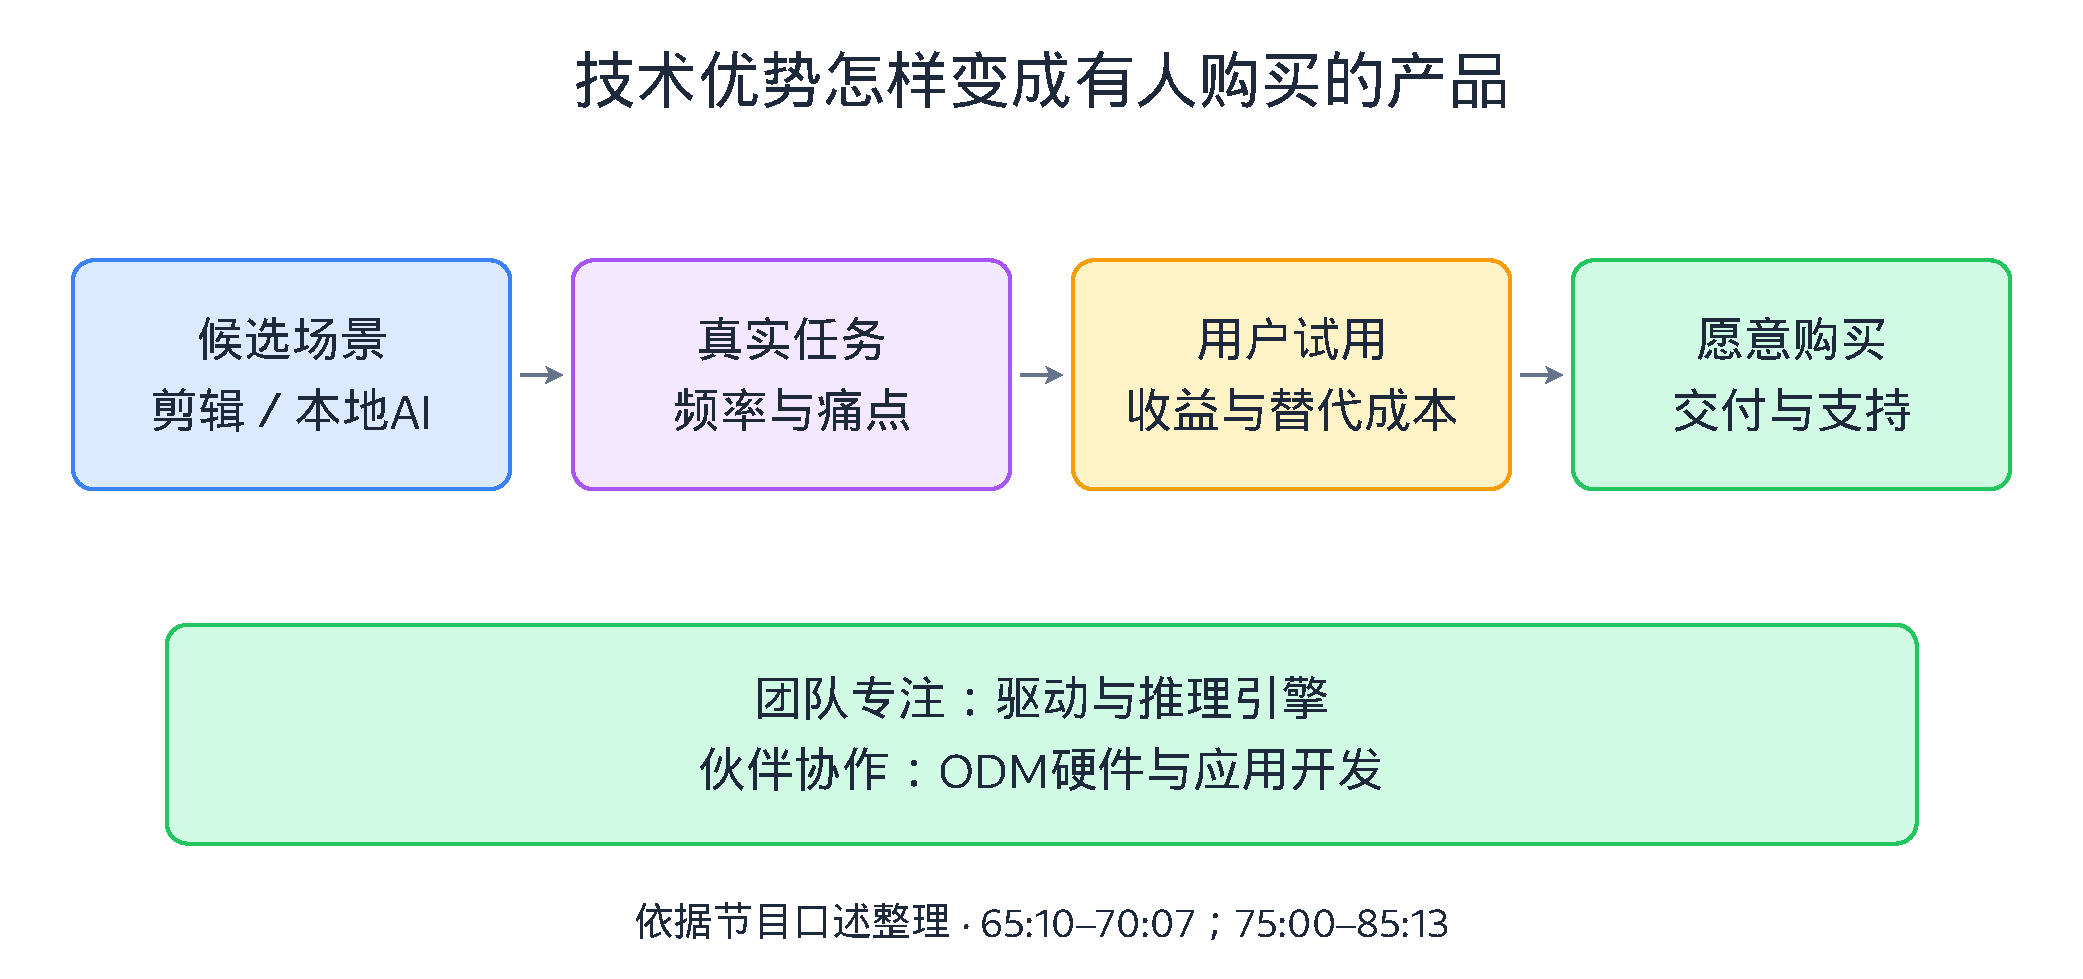
\includegraphics[width=\linewidth,height=.68\textheight,keepaspectratio]{assets/mechanism-06.pdf}
\caption{技术优势转化为购买决策与团队分工机制（依据节目口述整理 · 65:10–70:07；75:00–85:13）}
\end{figure}
\begin{knowledgebox}{读图：技术优势怎样变成有人购买的产品}
图中上方由左至右展示了将技术推向市场的四个递进环节：首先从“候选场景（剪辑／本地AI）”出发，进一步筛选“真实任务（频率与痛点）”，考察需求是否真实迫切；随后进入“用户试用（收益与替代成本）”环节，在市场试错中检验方案的实际价值；最终转化为“愿意购买（交付与支持）”。下方横跨全局的绿色底座标明了背后的组织分工：“团队专注：驱动与推理引擎”负责打造底层性能优势，“伙伴协作：ODM硬件与应用开发”负责承接硬件制造与上层应用探索。
\end{knowledgebox}
通过明确核心驱动层与外围生态的分工边界，并在真实市场中持续筛选有付费意愿的应用场景，初创团队才能将实验室里的体系结构积累逐步转化为商业产品。
\needspace{6\baselineskip}\subsection{本章小结}
\begin{enumerate}
\item 商业切入：区分“场景多”与“付费意愿多”，短期瞄准专业创作者、极客与小型工作室等“大C小B”群体作为切入口，在市场推广中持续试错，长期向家庭与办公算力中心演进。
\item 研发聚焦：团队专注Wi-Fi/GPU驱动、推理内核与推理引擎等底层基础设施，整机硬件交由ODM合作，上层应用联合开发者社区。
\item 持续创造：放小自我主动求助以打通小批量供应链，依托深圳硬件生态快速迭代，通过换位思考与对齐共同利益推进合作，并在长期奋斗中保持健康、享受当下过程。
\end{enumerate}
\needspace{8\baselineskip}\section{总结与延伸}
纵观孟子立从学术研究走向硬科技创业的历程，贯穿其中的是一套务实的系统工程思维。在科研层面，他看重从真实痛点（如视频通话卡顿、长走廊连续数门）出发定义问题，将算法视为服务于系统目标的可选工具，并在应用、传输、网络与链路的跨层协同中消解瓶颈。在决策与职业规划层面，他借用边际成本与边际收益权衡升学路径，把博士阶段作为有学位兜底的低成本试错窗口，在生产环境与商业场景的碰撞中认清“论文验证”与“产品交付”的距离。当角色延伸至高校导师与创业者后，面对AI工具对底层编码与信息载体的冲击，他主张将人才培养重心转向系统直觉、适应性与下限托底；而在推进无线算力原型WiCi时，则通过“核心驱动与推理层自研、整机硬件交由ODM、上层应用联合社区”的边界划分来集中有限资源。无论是主动求助打通深圳敏捷供应链，还是通过换位思考对齐各方共同利益，他都反复提醒同行：科研与创业是一场需要防范透支、保持健康并享受当下过程的持久战，最终追求的是做出真正留得下来的代表性工作。
\subsection{拓展阅读}
以下资料供回看节目、查阅术语与继续学习。
\begin{itemize}
\item 月球大叔：本期完整视频：\url{https://www.youtube.com/watch?v=c-MnSFGTSN8}
\item 官方完整逐字稿：\url{https://unclemoon.ai/blog/003-zili-meng/transcript/}
\item 官方访谈文章：\url{https://unclemoon.ai/blog/003-zili-meng/}
\end{itemize}
\end{document}
